Nesta secção irá ser abordado o estado da arte para a realização dos objetivos referidos na secção de introdução. 

O objetivo principal desta secção é descrever os conceitos e tecnologias usadas, tais como o \acrshort{jwt}, 
o Autenticação.gov, o \textit{Swagger}, entre outros. 

Além disso, pretende-se também fazer alguma investigação em termos de conversores de \acrshort{json} para 
\acrshort{xml} e de \acrshort{json} para \acrshort{csv} com o objetivo de averiguar aqueles que podem 
facilitar/ajudar na exportação de dados.

Por fim, são também investigados vários \textit{\acrshort{api} Gateways} para perceber aquele que suporta mais 
requisitos para simplificar a autenticação/proteção da \acrshort{api} de dados.

\section{\acrfull{jwt}}
O \acrshort{jwt} é um 
\textit{open standard}\footnote{Mais informação em \url{https://tools.ietf.org/html/rfc7519}} 
que define uma forma compacta e independente de transmitir com segurança informação entre partes com um objeto 
\acrshort{json}.~\cite{jwtio} 

O \acrshort{jwt} pode ser assinado digitalmente (\acrshort{jws}), encriptado (\acrshort{jwe}), assinado e depois 
encriptado (\acrshort{jws} encriptado, ou seja, um \acrshort{jwe}, ordem 
recomendada\footnote{Mais informação em \url{https://tools.ietf.org/html/rfc7519\#section-11.2}}) ou encriptado e 
depois assinado (\acrshort{jwe} assinado, ou seja, um \acrshort{jws}).

Caso seja assinado digitalmente é possível verificar a integridade da informação mas não é garantida a sua 
privacidade contudo podemos confiar na informação do \acrshort{jwt}. A assinatura pode ser efetuada através de 
um segredo usando por exemplo o algoritmo \acrshort{hmac} ou através de pares de chaves pública/privada usando 
por exemplo o algoritmo \acrshort{rsa}. No caso de se usar pares de chaves pública/privada a assinatura também 
garante que a parte envolvida que tem a chave privada é aquela que assinou o \acrshort{jwt}.

Por outro lado, os \acrshort{jwt}s podem ser encriptados garantindo a privacidade destes, escondendo a informação 
das partes não envolvidas. Nesta secção apenas se falará sobre \acrshort{jwt}s e \acrshort{jws}s (\acrshort{jwt} 
assinado). Se pretender saber mais sobre \acrshort{jwe}s pode ler o capítulo 5 do livro \textit{The JWT Handbook} 
por \textit{Sebastián E. Peyrott}.

Sendo assim, em que casos é útil o uso de \acrshort{jwt}s? 

Dois dos casos são os seguintes:
\begin{itemize}
    \item Autorização: Este será o caso para o qual o \acrshort{jwt} será usado na \acrshort{clav}. 
    Quando o utilizador realiza o \textit{login} gera-se um \acrshort{jwt} por forma a que os restantes pedidos 
    desse utilizador sejam realizados com esse \acrshort{jwt} (\acrlong{sso}). 
    O uso de \acrshort{jwt}s para estes casos permitem um \textit{overhead} pequeno e a flexibilidade de serem 
    usados em diferentes domínios;
    \item Troca de informação: No caso de troca de informação entre duas partes os \acrshort{jwt}s assinados são 
    de bastante utilidade visto que permitem verificar se o conteúdo não foi violado e, no caso de se usar pares 
    de chaves pública/privada para assinar, permitem ter a certeza que o remetente é quem diz ser.
\end{itemize}

\subsection{Estrutura do \acrshort{jwt}}

Os \acrshort{jwt}s são construídos a partir de três elementos, o \textit{header} (objeto \acrshort{json} também 
conhecido por \acrshort{jose} \textit{header}), o \textit{payload} (objeto \acrshort{json}) e os dados de 
assinatura/encriptação (depende do algoritmo usado). Estes elementos são depois codificados em representações 
compactas (\texttt{Base64 URL-safe}\footnote{Variante da codificação \texttt{Base64} onde a codificação gerada 
é segura para ser usada em \textit{URL}s. Basicamente para a codificação \texttt{Base64} gerada substitui os 
caracteres '+' e '/' pelos caracteres '-' e '\_' respetivamente. Além disso, remove o caractere de 
\textit{padding} e proíbe separadores de linha}). As codificações \texttt{Base64 URL-safe} de cada elemento 
são depois concatenadas numa \textit{string} onde é usado o caractere '.' para separar as partes, dando origem 
a uma representação final compacta do \acrshort{jwt} (\textit{JWS/JWE Compact Serialization}). 

Na secção~\ref{sec:criacaojwt} estão presentes dois diagramas referentes à construção de dois \acrshort{jwt}s 
sendo um deles assinado.

\begin{figure}[H]
    \centering
    \textbf{\textcolor{red}{eyJhbGciOiJIUzI1NiIsInR5cCI6IkpXVCJ9}.
        \textcolor{purple}{eyJuYW1lIjoiSm9zw6kgTWFydGlucyIsIm51bSI6ImE3ODgyMSJ9}.
        \textcolor{cyan}{tRPSYVsFI-nziRPuAjdGZLN2tUez5MtLML\_aAnPplgM}
    }
    \caption{Exemplo de representação compacta de \acrshort{jwt} (quebra de linhas por forma a melhorar leitura)}\label{fig:exemjwt}
\end{figure}

De seguida vamos aprofundar cada elemento referido:
\begin{itemize}
    \item[\textbf{\textit{Header}:}]

    O cabeçalho (a vermelho na figura~\ref{fig:exemjwt}) é constituído pelos seguintes atributos:
    \begin{itemize}
        \item O atributo obrigatório \texttt{alg} (algoritmo), único campo obrigatório para o caso de um 
        \acrshort{jwt} não encriptado, 
         onde é indicado que algoritmo é usado para assinar e/ou desencriptar. 
        O seu valor pode ser, por exemplo, HS256 (\acrshort{hmac} com o auxílio do 
        SHA-256\footnote{Função pertencente ao conjunto de funções \textit{hash} criptográficas 
        \acrfull{sha2} desenhadas pela \acrshort{nsa}}) ou \acrshort{rsa};
        \item O atributo opcional \texttt{typ} (tipo do \textit{token}) em que o seu valor é ``JWT''. 
        Serve apenas para distinguir os \acrshort{jwt}s de outros objetos que têm um \acrshort{jose} 
        \textit{header};
        \item O atributo opcional \texttt{cty} (tipo do conteúdo (\textit{payload})). 
        Se o \textit{payload} contiver atributos arbitrários este atributo não deve ser colocado. 
        Caso o \textit{payload} seja um \acrshort{jwt}\footnote{\acrshort{jwt} aninhado 
        (\textit{nested \acrshort{jwt}})} então este atributo deve ter o valor de ``JWT''.
    \end{itemize}

    O cabeçalho é de grande importância visto que permite saber se o \acrshort{jwt} é assinado ou encriptado e de 
    que forma o resto do \acrshort{jwt} deve ser interpretado.

    \begin{lstlisting}[language=json, caption=\textit{Header} usado para construir o \acrshort{jwt} da figura~\ref{fig:exemjwt}]
    {
        "alg": "HS256",
        "typ": "JWT"
    }
    \end{lstlisting}

    \item [\textbf{\textit{Payload}:}] O \textit{payload} (a roxo na figura~\ref{fig:exemjwt}) contém a 
    informação/dados que pretendemos transmitir com o \acrshort{jwt}. Não há atributos obrigatórios contudo 
    existem certos atributos que têm um significado definido (atributos registados).

    Existem 7 atributos registados (\textit{registered claims}):~\cite{jwthandbook}
    \begin{itemize}
        \item \texttt{iss} (\textit{issuer}): Identificador único (\textit{case-sensitive string}) que identifica 
        unicamente quem emitiu o \acrshort{jwt}. A sua interpretação é específica de cada aplicação visto que não há 
        uma autoridade central para gerir os emissores;
        \item \texttt{sub} (\textit{subject}): Identificador único (\textit{case-sensitive string}) que identifica 
        unicamente de quem é a informação que o \acrshort{jwt} transporta. Este atributo deve ser único no contexto 
        do emissor, ou se tal não for possível, globalmente único. O tratamento do atributo é específico a cada 
        aplicação;
        \item \texttt{aud} (\textit{audience}): Identificador único (\textit{case-sensitive string}) ou 
        \textit{array} destes identificadores únicos que identificam unicamente os destinatários pretendidos do 
        \acrshort{jwt}. Ou seja, quem lê o \acrshort{jwt} se não estiver no atributo \texttt{aud} não deve considerar 
        os dados contidos no \acrshort{jwt}. O tratamento deste atributo também é específico a cada aplicação; 
        \item \texttt{exp} (\textit{expiration (time)}): Um número inteiro que representa uma data e hora específicos 
        no formato \textit{seconds since epoch} definido pela 
        \acrshort{posix}\footnote{Mais informação em \url{https://pubs.opengroup.org/onlinepubs/9699919799/basedefs/V1\_chap04.html\#tag\_04\_16}}, 
        a partir da qual o \acrshort{jwt} é considerado inválido (expira);
        \item \texttt{nbf} (\textit{not before (time)}): Representa o inverso do atributo \texttt{exp} visto que é 
        um número inteiro que representa uma data e hora específicos no mesmo formato do atributo \texttt{exp}, mas 
        a partir da qual o \acrshort{jwt} é considerado válido;
        \item \texttt{iat} (\textit{issued at (time)}): Um número inteiro que representa uma data e hora especificos,
         no mesmo formato dos atributos \texttt{exp} e \texttt{nbf}, que representa o instante no qual o 
         \acrshort{jwt} foi emitido;
        \item \texttt{jti} (\textit{\acrshort{jwt} ID}): Identificador único (\textit{string}) do \acrshort{jwt} 
        que permite distinguir \acrshort{jwt}s com conteúdo semelhante. A implementação tem de garantir a unicidade 
        deste identificador.
    \end{itemize}

    Estes atributos registados têm todos 3 caracteres visto que um dos requisitos do \acrshort{jwt} é ser o mais 
    pequeno/compacto possível.

    Existem depois mais dois tipos de atributos, públicos e privados. 
    Os atributos públicos podem ser definidos à vontade pelos utilizadores de \acrshort{jwt}s mas têm de ser 
    registados em \textit{IANA JSON Web Token Claims registry} ou definidos por um espaço de nomes resistente 
    a colisões de forma a evitar a colisão de atributos. 
    Já os atributos privados são aqueles que não são nem registados nem públicos e podem ser definidos à vontade 
    pelos utilizadores de \acrshort{jwt}s. 
    Os dois atributos usados no exemplo~\ref{exem:pay} (\texttt{name} e \texttt{num}) são atributos privados.

    \begin{lstlisting}[language=json, caption=\textit{Payload} usado para construir o \acrshort{jwt} da figura~\ref{fig:exemjwt}, label=exem:pay]
    {
        "name": "José Martins",
        "num": "a78821"
    }
    \end{lstlisting}

\item [\textbf{\textit{Signature}:}] A assinatura (a azul na figura~\ref{fig:exemjwt}) é criada ao usar o 
algoritmo indicado na \textit{header} no atributo \texttt{alg} tendo como um dos argumentos os elementos 
codificados da \textit{header} e do \textit{payload} juntos por um ponto e como outro argumento um segredo. 
O resultado do algoritmo é depois codificado em \texttt{Base64 URL-safe}. 
Esta assinatura no caso dos \acrshort{jws}s é usada para verificar a integridade do \acrshort{jwt} e caso seja 
assinado com uma chave privada permite também verificar se o remetente é quem diz ser. 
No caso de o atributo \texttt{alg} for \texttt{none} a assinatura é uma \texttt{string} vazia.

    \begin{lstlisting}[language=javascript, caption=\textit{Signature} usado para construir o \acrshort{jwt} da figura~\ref{fig:exemjwt}]
    HMACSHA256(
        base64UrlEncode(header) + "." +
        base64UrlEncode(payload),
        segredo1.-uminho!clav
    )
    \end{lstlisting}
\end{itemize}

\subsection{Criação de \acrshort{jwt}/\acrshort{jws}}\label{sec:criacaojwt}

Na figura~\ref{fig:buildJWT} é apresentada a construção de um \acrshort{jwt} em que o atributo 
\texttt{alg} (algoritmo) tem o seu valor igual a \texttt{none}, ou seja, o \acrshort{jwt} não é 
assinado nem encriptado.

\begin{figure}[H]
    \centering
    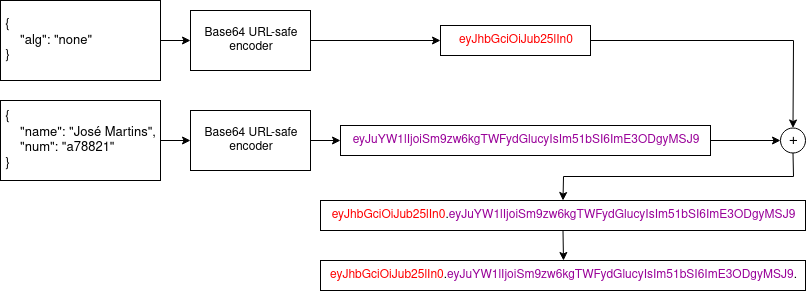
\includegraphics[width=1\textwidth]{img/buildJWT.png}
    \caption{Criação de um \acrshort{jwt}}\label{fig:buildJWT}
\end{figure}

Já na figura~\ref{fig:buildJWS} é demonstrada a construção de um \acrshort{jwt} assinado, ou seja, um \acrshort{jws}.

\begin{figure}[H]
    \centering
    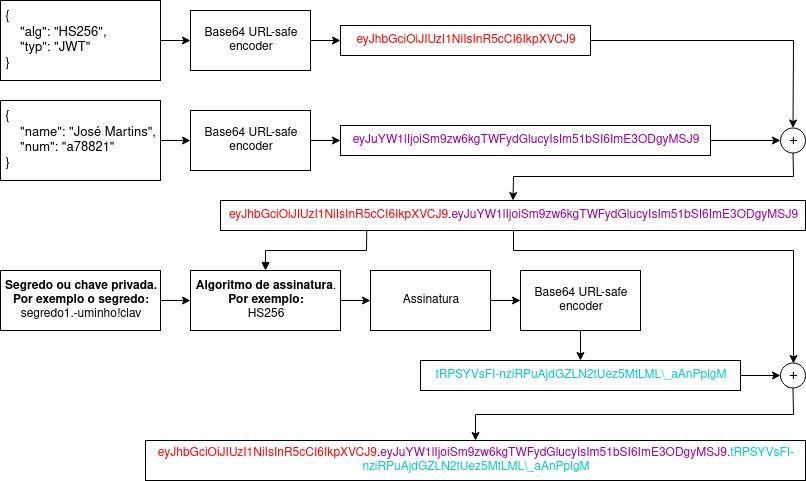
\includegraphics[width=1\textwidth]{img/buildJWS.png}
    \caption{Criação de um \acrshort{jws}}\label{fig:buildJWS}
\end{figure}

\subsection{Alternativas ao \acrshort{jwt}}

Algumas alternativas ao \acrshort{jwt} passam pelo uso de \acrfull{swt} ou \acrfull{saml}. 
Se compararmos o \acrshort{jwt} ao \acrshort{saml}, o \acrshort{json} é menos verboso que o 
\acrshort{xml} e mesmo quando codificado o seu tamanho é menor. 

De um ponto de vista de segurança o \acrshort{swt} apenas pode ser assinado simetricamente por um segredo 
partilhado usando o algoritmo \acrshort{hmac}. Já o \acrshort{jwt} e o \acrshort{saml} podem usar pares de 
chaves pública/privada para assinar. Contudo assinar \acrshort{xml} com 
\textit{\acrshort{xml} Digital Signature} sem introduzir buracos de segurança é mais difícil quando comparado 
com a simplicidade de assinar \acrshort{json}.~\cite{jwtio}

Houve contudo algumas bibliotecas de \acrshort{jwt} com vulnerabilidades devido ao atributo \texttt{alg} da 
\textit{header} do \acrshort{jwt}. Havia duas situações de vulnerabilidade:
\begin{itemize}
    \item As bibliotecas ao fazer a verificação (recebe um \acrshort{jwt} e um segredo/chave pública como 
    argumentos) de um \acrshort{jwt} com \texttt{alg} igual a \texttt{none} assumiam logo que o \acrshort{jwt} 
    era válido mesmo que o segredo/chave pública fosse diferente de vazio. Ou seja, com a simples alteração do 
    atributo \texttt{alg} e com a remoção da \textit{signature} podia-se alterar o \textit{payload} do 
    \acrshort{jwt} que o servidor iria continuar a considerar que a integridade do \acrshort{jwt} não foi colocada 
    em causa mesmo que os \acrshort{jwt}s gerados pelo servidor tivessem sido assinados com um algoritmo e 
    com recurso 
    a um segredo/chave privada;

    \item As bibliotecas ao fazer a verificação seja de um algoritmo simétrico ou assimétrico apenas tinham 
    como parâmetros o \acrshort{jwt} e o segredo/chave pública. Isto gera uma segunda vulnerabilidade. Se o 
    servidor estiver à espera de um \acrshort{jwt} assinado com pares de chaves pública/privada mas receber 
    um \acrshort{jwt} assinado com \acrshort{hmac} vai assumir que a chave pública é o segredo a usar no algoritmo 
    \acrshort{hmac}. Ou seja, se se criar um \acrshort{jwt} com o atributo \texttt{alg} igual a \acrshort{hmac} 
    e a assinatura for gerada usando o algoritmo \acrshort{hmac} com o segredo a ser a chave pública, podemos 
    alterar o \textit{payload} (antes de assinar) que o servidor vai considerar que o \acrshort{jwt} não foi 
    maliciosamente alterado.
\end{itemize}

Portanto a flexibilidade de algoritmos dada pelo \acrshort{jwt} coloca em causa a segurança pelo que da parte das 
bibliotecas o atributo \texttt{alg} não deve ser considerado~\cite{jwtvuln} bem como deve ser \textit{deprecated} 
e deixar de ser incluído nos 
\acrshort{jwt}s\footnote{Ver \url{https://gist.github.com/paragonie-scott/c88290347c2589b0cd38d8bb6ac27c03}}. 

A biblioteca que será usada na \acrshort{clav}, 
\texttt{jsonwebtoken}\footnote{Ver \url{https://www.npmjs.com/package/jsonwebtoken}}, já endereçou estes 
problemas\footnote{Ver \url{https://github.com/auth0/node-jsonwebtoken/commit/1bb584bc382295eeb7ee8c4452a673a77a68b687}} 
pelo que estas vulnerabilidades não estarão presentes na \acrshort{clav}.

Ainda comparando as diferentes alternativas, os \textit{parsers} de \acrshort{json} são mais comuns em grande 
parte das linguagens de programação visto que os \acrshort{json}s mapeiam diretamente para objetos ao contrário 
do \acrshort{xml} que não tem um mapeamento natural de documento para objeto.~\cite{jwtio} 
Isto torna mais fácil trabalhar com \acrshort{jwt} do que com \acrshort{saml}.

Já quando comparamos os \acrshort{jwt}s a \textit{cookie sessions}, o \acrshort{jwt} tem a vantagem de as sessões 
puderem ser \textit{stateless} enquanto que as \textit{cookies} são \textit{statefull}. Contudo, 
ser \textit{stateless} não permite por exemplo que a qualquer altura se possa revogar um \acrshort{jwt}. 
Para endereçar esse problema é necessário, por exemplo, guardar (\textit{statefull}) os \acrshort{jwt}s numa base 
de dados associando cada \acrshort{jwt} ao identificador único de quem é a informação contida no \acrshort{jwt} 
(o uso de uma \textit{whitelist}). Assim para revogar um \acrshort{jwt} bastaria removê-lo da base de dados.

Outra alternativa ao \acrshort{jwt} seria \textit{sessionIDs}. As \textit{sessionIDs} são \textit{strings} longas, 
únicas e aleatórias. É possível revogar um \textit{sessionID}, ao contrário do \acrshort{jwt}, bastando para isso 
remover o \textit{sessionID} da base de dados.

Por fim, uma outra alternativa bastante semelhante ao \acrshort{jwt} é \textit{Branca}. 
\textit{Branca} usa o algoritmo simétrico \textit{\acrshort{ietf} XChaCha20-Poly1305 \acrshort{aead}} que permite 
criar \textit{tokens} encriptados com a garantia de integridade. Tem também uma região de \textit{payload} como 
\acrshort{jwt} com a única diferença é que este \textit{payload} não tem uma estrutura definida. Não necessita da 
\textit{header} visto que o algoritmo usado não varia. Em vez de usar codificação em \texttt{Base64 URL-safe} 
usa \texttt{Base62} que também é \textit{URL-safe}. Para além disso o \textit{token} gerado é geralmente de menor 
dimensão do que o gerado pelo \acrshort{jwt} sendo como tal mais compacto que o \acrshort{jwt}.~\cite{branca} 
Visto que o \textit{Branca} encripta e garante integridade de uma forma mais simples que o \acrshort{jwt} 
permite (para isso era necessário recorrer a um \acrshort{jwe} que tem no seu \textit{payload} um \acrshort{jws}), 
sendo como tal propenso a menos erros de programação. 
Contudo, o \textit{Branca} ainda não é muito conhecido nem um \textit{standard} da indústria, ao contrário do 
\acrshort{jwt}, mas não deixa de ser algo a ter em conta para o futuro. 

\section{Autenticação.gov}
O Autenticação.gov surgiu da necessidade de identificação unívoca de um utilizador perante sítios na 
Web.~\cite{agov} Será este componente a realizar o processo de autenticação do utilizador e a fornecer
 os atributos do utilizador necessários para identificar o utilizador numa entidade (\textit{website}/portal).

O \acrshort{cc} em conjunto com o Autenticação.gov permite obter os identificadores dos utilizadores junto das 
entidades participantes da iniciativa do \acrshort{cc} (funcionalidade de Federação de Identidades da Plataforma 
de Interoperabilidade da Administração Pública). Além disso, o Autenticação.gov gere os vários fornecedores de 
atributos disponíveis bem como possui uma estreita ligação com a infraestrutura de chave pública do \acrlong{cc} 
(\acrfull{pki}), com o intuito de manter os elevados níveis de segurança e privacidade no processo de autenticação 
e identificação.~\cite{agov}

O Autenticação.gov permite também a criação de credenciais comuns a todos os sites da \acrshort{ap}, ou seja, 
o utilizador apenas necessita de se autenticar uma vez que poderá aceder aos vários portais (Portal do Cidadão, 
etc) com a mesma autenticação (\acrshort{sso}).

Para além disso o utilizador pode autenticar-se utilizando outros certificados digitais que não o \acrshort{cc} 
(por exemplo \acrfull{cmd}, \textit{user+password} ou redes sociais, estes dois últimos quando o 
\textit{website}/portal necessita apenas de conhecer do utilizador o \textit{email}).

No projeto \acrshort{clav} irá ser implementado a autenticação com recurso ao Autenticação.gov através de dois 
certificados digitais diferentes:
\begin{itemize}
    \item \acrfull{cc}: Já se encontra implementado como referido na secção~\ref{sec:autenticacao}. 
    A autenticação é realizada através da leitura do \acrshort{cc} (através de um leitor de cartões sendo 
    necessário a instalação de \textit{software} do Autenticação.gov para proceder à leitura do \acrshort{cc}) e 
    posterior inserção do \acrshort{pin} de autenticação recebido quando se cria/renova o \acrshort{cc};

    \item \acrfull{cmd}: Um dos objetivos desta tese é a implementação da autenticação com recurso a este 
    certificado digital. Com o \acrshort{cmd}, após o utilizador associar um número de telemóvel ao 
    \acrshort{nic}, o utilizador pode autenticar-se com o número de telemóvel, o código \acrshort{pin} da 
    \acrshort{cmd} e o código de segurança temporário enviado por \acrshort{sms}.
\end{itemize}

De forma a completar a figura~\ref{fig:authgov} apresenta-se de seguida, na figura~\ref{fig:fluxoauthgov}, o fluxo de pedidos efetuado entre 
a \acrshort{clav} e o Autenticação.gov de forma a autenticar um utilizador na \acrshort{clav}:~\cite{agov}
\begin{figure}[H]
    \centering
    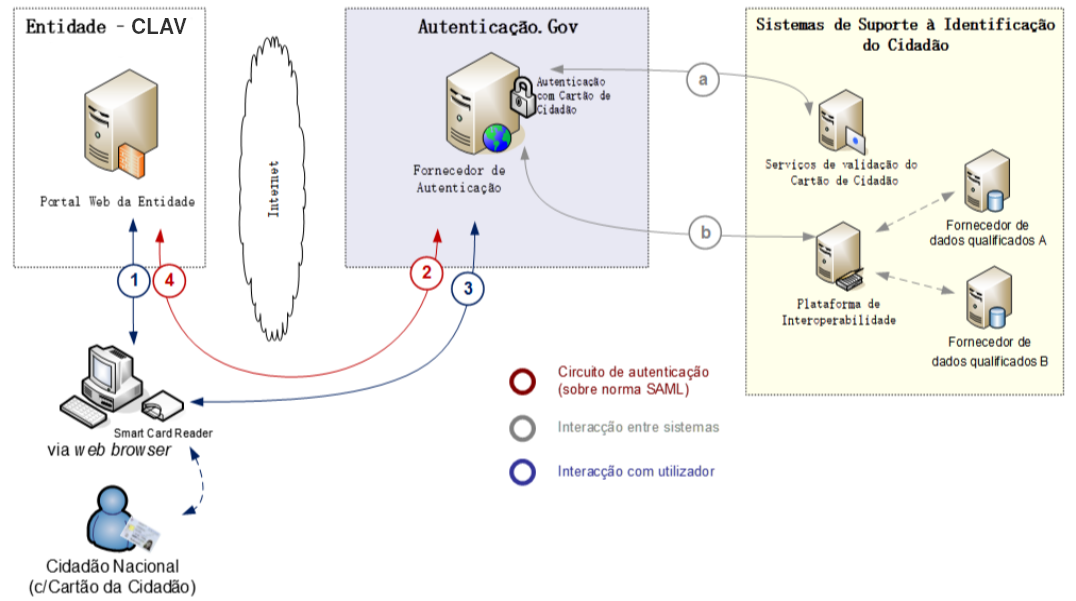
\includegraphics[width=1\textwidth]{img/fluxoauthgov.png}
    \caption{Fluxo de pedidos entre a \acrshort{clav} e o Autenticação.gov de forma a autenticar um utilizador na \acrshort{clav}.~\cite{agov}}\label{fig:fluxoauthgov}
\end{figure}

\begin{enumerate}
    \item O utilizador pretende aceder à área privada do portal de uma entidade (da \acrshort{clav}), na qual 
    é necessário que comprove a sua identidade;
    \item O portal da entidade (\acrshort{clav}) delega a autenticação e redireciona o utilizador para o 
    Autenticação.gov, juntamente com um pedido de autenticação assinado digitalmente;
    \item O Autenticação.gov valida o pedido de autenticação recebido e solicita a autenticação do utilizador 
    com recurso ao seu \acrshort{cc} pedindo a inserção do seu \acrshort{pin} de autenticação. 
    Durante este processo, o Autenticação.gov efetua as seguintes operações internas:
    \begin{enumerate}
        \item Valida as credenciais do utilizador com recurso à \acrshort{pki} do \acrshort{cc} 
        via \acrshort{ocsp};
        \item Obtém atributos que sejam solicitados pelo portal da entidade (\acrshort{clav}) junto dos vários 
        fornecedores de atributos qualificados. Esta operação é efetuada via Plataforma de Interoperabilidade. 
        Este processo pode incluir a obtenção de dados da Federação de Identidades ou de outras Entidades.
    \end{enumerate}

    \item A identificação e atributos do utilizador são autenticados e assinados digitalmente pelo 
    Autenticação.gov, após o qual redireciona o utilizador de volta ao portal da entidade original (\acrshort{clav}). Cabe à entidade (\acrshort{clav}) a validação das credenciais do Autenticação.gov e utilização dos atributos do cidadão.
\end{enumerate}

A troca de pedidos entre a \acrshort{clav} e o Autenticação.gov é feita através de \acrshort{saml} 2.0.

O \acrfull{saml} define uma \textit{framework} \textit{standard} em \acrshort{xml}.~\cite{sam2man} 
Foi aprovado pela \acrshort{oasis}, permite a troca segura de informação de autenticação e autorização entre 
diferentes entidades possibilitando através de uma credencial (\textit{login} de um utilizador) aceder autenticado 
a um conjunto de \textit{websites} (\acrshort{sso}).

Para utilizar o Autenticação.gov é necessário criar um pedido baseado em \acrshort{saml}, assinado digitalmente 
com um certificado X.509 (permite ao Autenticação.gov identificar a entidade responsável pelo pedido) e encriptado 
com a chave privada de um par de chaves \acrshort{rsa} (permite ao Autenticação.gov verificar a validade do 
pedido de autenticação), bem como a respetiva cadeia de autenticação.~\cite{otavioTese} 
A chave pública do par de chaves \acrshort{rsa} faz parte do certificado X.509 que é enviado ao Autenticação.gov.

Há dois tipos de \acrshort{saml} usados com o Autenticação.gov~\cite{otavioTese}:
\begin{itemize}
    \item \textbf{\acrshort{saml} Request (2 da figura~\ref{fig:fluxoauthgov}):} Pedido de autenticação, 
    enviado ao Autenticação.gov, no qual é enviado a origem, assinaturas, atributos a obter do utilizador, etc.
    \item \textbf{\acrshort{saml} Response (4 da figura~\ref{fig:fluxoauthgov}):} Resposta ao pedido de 
    autenticação enviado para o \textit{issuer} do pedido de autenticação. Esta resposta contém o 
    \textit{status} do pedido de autenticação (sucesso, insucesso ou cancelado) e no caso de uma autenticação 
    com sucesso contém os atributos do utilizador requisitados.
\end{itemize}

Tanto o pedido e a resposta estão no formato \acrshort{xml} pelo simples facto de ser usado o \acrshort{saml} 2.0.

No caso do \textit{\acrshort{saml} Request} o pedido possui o elemento \textit{root} \texttt{AuthnRequest} onde 
se destacam os seguintes atributos:
\begin{itemize}
    \item \textbf{Destination}: \acrshort{url} para o qual o pedido de autenticação é enviado. No caso da 
    Autenticação.gov este apenas pode ser um dos seguintes \acrshort{url}'s:
    \begin{itemize}
        \item \url{https://preprod.autenticacao.gov.pt/fa/Default.aspx} para o ambiente de teste;
        \item \url{https://autenticacao.gov.pt/fa/Default.aspx} para o ambiente de produção 
        (obrigatório o uso de \acrshort{https} para a comunicação).
    \end{itemize}
    \item \textbf{AssertionConsumerServiceURL}: \acrshort{url} destino da resposta do pedido de autenticação 
    (\textit{\acrshort{saml} Response}). Em produção, é obrigatório que o \acrshort{url} seja em \acrshort{https};
    \item \textbf{ProviderName}: Nome da plataforma/aplicação que está a requerer a autenticação através do 
    Autenticação.gov. Este nome tem de ser previamente acordado com a \acrshort{ama} durante a emissão da cadeia 
    de autenticação e certificados X.509~\cite{otavioTese}.
\end{itemize}

Além destes atributos, o \textit{\acrshort{saml} Request} possui 3 elementos aninhados:\label{sec:soaAuthCMDReq}
\begin{itemize}
    \item \textbf{Issuer}: Informação sobre quem efetua o pedido de autenticação, ou seja a \acrshort{clav}. 
    Basta apenas enviar o \acrshort{url} de onde é originário o pedido;
    \item \textbf{Signature}: Assinatura digital do pedido. Aqui é adicionado o certificado X.509 com a cadeia de 
    autenticação fornecida pela \acrshort{ama};
    \item \textbf{Extensions}: Contém os atributos a requisitar ao Autenticação.gov do utilizador a autenticar-se 
    na \acrshort{clav}. Aqui são também adicionados o nível de confiança e a política de apresentação do 
    Autenticação.gov:
    \begin{itemize}
        \item \textbf{Nível de confiança} \\
        Permite indicar o nível mínimo necessário para realizar a autenticação. Os níveis passíveis de usar 
        são~\cite{agov2}:
        \begin{itemize}
            \item 4:
            \begin{itemize}
                \item Autenticação com recurso a uma ou mais operações criptográficas efetuadas no \acrlong{cc} 
                em autenticação que resulta num conjunto de informação fornecida ao Autenticação.gov que permite 
                com o maior grau de certeza de que, no momento da autenticação, se utilizou um \acrlong{cc} real 
                com conhecimento do \acrshort{pin} de autenticação;
                \item Autenticação com renegociação \acrshort{ssl} com certificado cliente da Ordem dos Notários, 
                da Ordem dos Advogados ou da Câmara dos Solicitadores;
            \end{itemize}
            \item 3: Autenticação com \acrlong{cmd};
            \item 2: Autenticação com \acrlong{cmd} através de Email ou \textit{Twitter};
            \item 1: Autenticação com Utilizador/Palavra-passe (também designado por Autenticação Simples) e 
            Redes Sociais.
        \end{itemize}
        \item \textbf{Política de apresentação} \\
        No Autenticação.gov quando o nível de confiança é inferior a 4 são apresentadas múltiplas abas com os 
        Mecanismos de Autenticação disponíveis. A política de apresentação permite definir o que deve ou não ser 
        apresentado (que abas devem estar disponíveis tendo em conta o nível de confiança definido) e/ou que 
        método de autenticação (aba) deve ser o predefinido. Em caso de conflitos entre o nível de confiança e a 
        política de apresentação ou conflitos na própria política de apresentação, esta é ignorada e é utilizada 
        a política de apresentação que privilegia o \acrshort{cc} (mecanismo de autenticação mais seguro). 
        Os Mecanismos de Autenticação disponíveis são~\cite{agov2}:
            \begin{itemize}
                \item \acrlong{cc};
                \item \acrlong{cmd};
                \item Utilizador/Palavra-passe também designado por Autenticação Simples;
                \item Redes Sociais.
            \end{itemize}
            E o mapeamento das abas aos mecanismos de autenticação é~\cite{agov2}:
            \begin{itemize}
                \item 'CC': Aba relativa à autenticação através de \acrlong{cc};
                \item 'CMD': Aba relativa à autenticação através de \acrlong{cmd};
                \item 'UPP': Aba relativa à autenticação através de Utilizador/Palavra-passe;
                \item 'RSS': Aba relativa à autenticação através das Redes Sociais.
            \end{itemize}
            Esta identificação é usada para identificar as abas na extensão em XML.
    \end{itemize}
\end{itemize}

Após a receção do \textit{\acrshort{saml} Request}, o Autenticação.gov processa a autenticação do utilizador 
e retorna o \textit{\acrshort{saml} Response} como resposta.

O \textit{\acrshort{saml} Response} tem como elemento \textit{root} \textit{Response}.
Este elemento possui 5 elementos aninhados dos quais se destaca:
\begin{itemize}
    \item \textbf{Status}: Contém a informação relativa ao sucesso ou insucesso do pedido de autenticação;
    \item \textbf{Assertion}: Asserção \acrshort{saml} que contém os atributos requisitados sobre o utilizador 
    no caso do pedido de autenticação ter sucesso.
\end{itemize}

Para finalizar é importante referir que o Autenticação.gov é como se fosse uma caixa negra à qual é enviado um 
pedido pela entidade que necessita a autenticação do utilizador (neste caso a \acrshort{clav}) com algumas 
configurações a usar pelo Autenticação.gov e, esta caixa negra, devolve a informação do utilizador autenticado 
(os atributos do utilizador requisitados no pedido efetuado ao Autenticação.gov). Os atributos são apenas 
devolvidos à entidade caso o utilizador autorize o Autenticação.gov a dar à entidade essa informação. 
A caixa negra trata de autenticar o utilizador através das credenciais fornecidas por este.

Para um maior aprofundamento sobre o Autenticação.gov recomenda-se a leitura da secção 2.2 da 
dissertação~\cite{otavioTese} (``CLAV: Autenticação e integração na plataforma iAP'' de Octávio Maia).

\section{Swagger}
O \textit{Swagger} é um ecossistema de ferramentas para desenvolver \acrshort{api}s com a \acrfull{oas}.

Até 2015 o \textit{Swagger} consistia numa especificação e num ecossistema de ferramentas para implementar a 
especificação. Em 2015 a fundadora do \textit{Swagger}, \textit{SmartBear Software}, doou a especificação 
\textit{Swagger} para a \textit{Linux Foundation} e renomeou a especificação para \acrlong{oas}.~\cite{wiswagger}

A especificação \textit{OpenAPI} é agora desenvolvida pela \textit{OpenAPI Initiative} que envolve várias 
empresas tecnológicas entre as quais \textit{Microsoft}, \textit{Google}, \textit{IBM} e a 
fundadora \textit{Smartbear Software}.

Já o conjunto de ferramentas \textit{Swagger} inclui ferramentas \textit{open-source}, gratuitas e comerciais 
que podem ser usadas em diferentes estágios do ciclo de vida de uma \acrshort{api}, que inclui documentação, 
desenho, testes e \textit{deployment}. Algumas das ferramentas são:~\cite{swaggerVSoas}
\begin{itemize}
    \item \textbf{\textit{Swagger Editor}}: Permite editar especificações \textit{OpenAPI} em 
    \acrshort{yaml} no \textit{browser}\footnote{Aceder \url{https://editor.swagger.io/}}, 
    validar as especificações em relação às regras do \acrshort{oas} bem como pré-visualizar 
    a documentação em tempo real. Facilita o desenho e a documentação de \acrshort{api}s \acrshort{rest};

    \item \textbf{\textit{Swagger \acrshort{ui}}}: Coleção de \textit{assets} \textit{\acrshort{html}}, 
    \textit{JavaScript} e \textit{\acrshort{css}} que geram dinamicamente documentação a partir de uma 
    especificação \textit{OpenAPI} de uma \acrshort{api};

    \item \textbf{\textit{Swagger Codegen}}: Permite a geração de bibliotecas cliente (geração de \acrshort{sdk}), 
    \textit{server stubs} e documentação automática a partir de especificações \textit{OpenAPI};

    \item \textbf{\textit{Swagger Inspector}}: Ferramenta de testes de \acrshort{api}s que permite validar 
    as \acrshort{api}s e gerar definições \textit{OpenAPI} de \acrshort{api}s existentes;

    \item \textbf{\textit{SwaggerHub}}: Desenho e documentação de \acrshort{api}s, construído para equipas que 
    trabalham com \textit{OpenAPI}.
\end{itemize}

O \textit{Swagger} possui duas abordagens:~\cite{swaggerNode}
\begin{itemize}
    \item \textit{top-down}: Uso do \textit{Swagger Editor} para criar a especificação \textit{OpenAPI} e 
    depois usar o \textit{Swagger Codegen} por forma a gerar o código do cliente e do servidor. Ou seja, 
    primeiro desenha-se a \acrshort{api} antes de escrever código;

    \item \textit{bottom-up}: Utilizador já possui uma \acrshort{api} \acrshort{rest} e o \textit{Swagger} irá 
    ser usado apenas para documentar a \acrshort{api} existente.
\end{itemize}

Visto que a \acrshort{clav} já possui grande parte da \acrshort{api} construída vai ser usada uma abordagem 
\textit{bottom-up}. Portanto, o \textit{Swagger} vai ser usado apenas para a documentação da \acrshort{api}. 
De forma a produzir a documentação, do portfólio de ferramentas do \textit{Swagger} apenas precisaremos de 
utilizar o \textit{Swagger \acrshort{ui}} e o \textit{Swagger Editor}. O primeiro permitirá apresentar aos 
utilizadores a documentação gerada e o segundo permitirá validar a especificação \textit{OpenAPI} (documentação) 
criada, verificando se não possui erros.

\subsection{Especificação \textit{OpenAPI}}

A especificação \textit{OpenAPI} providencia um conjunto de propriedades que podem ser usadas para descrever 
uma \acrshort{api} \acrshort{rest}. Com um documento de especificação válido é possível usá-lo para criar uma 
documentação interativa, por exemplo, através do \textit{Swagger \acrshort{ui}}.

De seguida será apresentado o que é possível documentar com a especificação \textit{OpenAPI} e como. 
É possível usar tanto \acrshort{yaml} como \acrshort{json} para a especificar. Esta parte será demonstrada 
usando \acrshort{yaml}.\footnote{A especificação completa do \textit{OpenAPI} com versão igual a 3.0.0 pode 
ser vista em \url{https://github.com/OAI/OpenAPI-Specification/blob/master/versions/3.0.0.md}}

\subsubsection{Metadata}
O primeiro passo é escolher a versão da especificação \textit{OpenAPI} que irá ser usada para documentar:
\begin{lstlisting}[language=yaml, caption=Exemplo de indicação da versão da especificação \textit{OpenAPI}]
openapi: 3.0.0
\end{lstlisting}

Depois, na secção \texttt{info}, é possível descrever um pouco a \acrshort{api} que estamos a documentar, 
indicando o título, a descrição e a versão da mesma. As propriedades \texttt{title} e \texttt{version} são 
obrigatórias. É possível também colocar informação sobre os contactos disponíveis, termos de uso e a 
licença:\footnote{Ver mais em \url{https://github.com/OAI/OpenAPI-Specification/blob/master/versions/3.0.0.md\#infoObject}}
\begin{lstlisting}[language=yaml, caption={Exemplo de secção \texttt{info} indicando título, descrição e versão da \acrshort{api} na especificação \textit{OpenAPI}}]
info:
  title: CLAV API
  description: Esta é a API do projeto CLAV...
  version: 1.0.0
\end{lstlisting}

\vspace{-0.7cm}

\subsubsection{Servidores}
Há depois uma secção com o nome de \texttt{servers} para indicar os \textit{URL}s que são os pontos de acesso 
da \acrshort{api}. Podem ser indicados vários pontos de 
acesso:\footnote{Para mais detalhes sobre esta secção veja \url{https://swagger.io/docs/specification/api-host-and-base-path/}}
\begin{lstlisting}[language=yaml, caption=Exemplo de secção \texttt{servers} indicando os \textit{URL}s e a descrição de cada na especificação \textit{OpenAPI}]
servers:
  - url: http://clav-api.dglab.gov.pt/api
    description: Official API server
  - url: http://clav-test.di.uminho.pt/api
    description: Testing server
  - url: http://localhost:7779/api
    description: Local server
\end{lstlisting}

\vspace{-0.7cm}

\subsubsection{Caminhos/Rotas}
De seguida apresenta-se uma das secções mais importantes da especificação, a secção \texttt{paths}. 
Aqui são definidas as rotas que a \acrshort{api} disponibiliza. Para definir cada rota basta indicar o caminho 
relativo aos pontos de acesso definidos na secção \texttt{servers} (\verb|<server-url>/<caminho relativo>|). 
Nesta secção é definido tudo o que envolve as rotas, desde os parâmetros necessários, as respostas que devolve, 
os métodos \textit{HTTP} disponíveis, etc:\footnote{Mais detalhes em \url{https://swagger.io/docs/specification/paths-and-operations/}}\footnote{mais detalhes sobre a funcionalidade \texttt{\$ref} em \url{https://swagger.io/docs/specification/using-ref/}}
\begin{lstlisting}[language=yaml, caption=Exemplo de secção \texttt{paths} indicando os detalhes de cada rota na especificação \textit{OpenAPI}, label={exem:oapiRota}]
paths:
  /users/{id}:
    get:
      summary: Resumo do que faz a rota
      description: >
        Descrição detalhada, pode ser usado Markdown para enriquecer o texto
      parameters:
        - name: id
          in: path
          description: Id do utilizador
          required: true
          schema:
            type: string
      responses:
        200:
          description: Descrição da resposta, p.e: Sucesso
          content:
            application/json:
              schema:
                #A estrutura do JSON devolvido pode ser definido logo aqui ou num componente à parte, fazendo referência desse. Iremos aplicar o segundo caso para demonstrar que estas funcionalidades tornam a documentação mais fácil de manter
                $ref: '#/components/schemas/User'
    post:
      ...
    delete:
      ...
  /users:
    ...

components:
  schemas:
    User:
      type: object
      properties:
        id:
          type: string
        ...
      required:
        - id
        ...
\end{lstlisting}

Outro ponto importante a referir é que é possível agrupar as rotas em grupos através do uso de \textit{tags}. 
As \textit{tags} têm de ser definidas numa secção chamada \textit{tags}:
\begin{lstlisting}[language=yaml, caption={Exemplo de secção \texttt{tags} definindo tags na especificação \textit{OpenAPI}}]
tags:
  - name: users
    description: Descrição
  - name: classes
    description: Outra descrição
\end{lstlisting}

Depois em cada rota é necessário indicar a que \textit{tag} (grupo) pertence:
\begin{lstlisting}[language=yaml, caption=Exemplo de uso de \textit{tags} numa rota na especificação \textit{OpenAPI}]
paths:
  /users/{id}:
    get:
      summary: Resumo do que faz a rota
      tags:
        - users
      ...
\end{lstlisting}

\vspace{-0.7cm}

\subsubsection{Parâmetros}\label{sec:paramSwagger}
Como já exemplificado no exemplo~\ref{exem:oapiRota} os parâmetros de uma rota são definidos na 
secção \texttt{parameters} de cada rota. 
Existem quatro tipo de parâmetros que variam de acordo com o local onde se encontram. 
O tipo de um parâmetro é definido na propriedade \texttt{in} de um parâmetro e pode ser um dos seguintes:
\begin{itemize}
    \item Parâmetros no caminho: Servem normalmente para apontar para um recurso específico. 
    Estes parâmetros são sempre obrigatórios como tal a propriedade \texttt{required} com o valor igual a 
    verdadeiro deve ser sempre adicionada. Para além disso o \texttt{name} tem de ser igual ao que está no 
    caminho. A propriedade \texttt{in} tem o valor de \textit{path};
    \item Parâmetros na \textit{query string}: A propriedade \texttt{in} tem o valor de \textit{query}. 
    No caso de tokens passados em parâmetros da \textit{query string} devem-se usar esquemas de segurança, 
    veja a secção~\ref{sec:authSwagger} Autenticação;
    \item Parâmetros no cabeçalho: A propriedade \texttt{in} tem o valor de \textit{header}. 
    Contudo os cabeçalhos \textit{Accept}, \textit{Content-Type} e \textit{Authorization} não são aqui definidos;
    \item Parâmetros no cabeçalho da \textit{Cookie}: A propriedade \texttt{in} tem o valor de \textit{cookie}.
\end{itemize}

Cada parâmetro tem várias propriedades que permitem defini-lo:\footnote{Mais detalhes em \url{https://swagger.io/docs/specification/describing-parameters/}}
\begin{itemize}
    \item \texttt{required}: Indica se o parâmetro é obrigatório ou opcional. 
    Possíveis valores são \textit{true} ou \textit{false}.
    \item \texttt{schema}:
    \begin{itemize}
        \item \texttt{default}: Valor padrão de um parâmetro opcional;
        \item \texttt{type}: O tipo do parâmetro. Possíveis valores: \textit{string}, \textit{integer}, etc;
        \item \texttt{enum}: Indica os possíveis valores para o parâmetro;
        \item \texttt{nullable}: Indica se o parâmetro pode ser \textit{null}. Possíveis valores são 
        \textit{true} ou \textit{false}.
    \end{itemize}
    \item \texttt{allowEmptyValue}: Indica se o parâmetro pode ser vazio. Apenas aplicável no caso de um 
    parâmetro na \textit{query string}. Possíveis valores são \textit{true} ou \textit{false};
    \item \texttt{example}: Um exemplo do valor;
    \item \texttt{examples}: Múltiplos exemplos;
    \item \texttt{deprecated}: Indica se o parâmetro é ou não \textit{deprecated}. Possíveis valores são 
    \textit{true} ou \textit{false}.
\end{itemize}

\subsubsection{\textit{Request Body}}
O \textit{request body} é definido em cada rota na secção \texttt{requestBody} sendo usado essencialmente em 
rotas com o método \acrshort{http} igual a POST ou a PUT, ou seja, em casos que há necessidade de criar ou alterar 
um objeto de acordo com a informação fornecida no pedido. As propriedades que podem ser definidas no 
\texttt{requestBody} são as seguintes:\footnote{Para mais detalhes, desde \textit{upload} de ficheiros, a \textit{Form Data}s, veja em \url{https://swagger.io/docs/specification/describing-request-body/}}\footnote{Para mais informação sobre os \textit{media types} veja \url{https://swagger.io/docs/specification/media-types/}}
\begin{itemize}
    \item \texttt{description}: Opcionalmente pode ser adicionada uma descrição;
    \item \texttt{required}: Indica se o \textit{request body} é obrigatório ou opcional. 
    Possíveis valores são \textit{true} ou \textit{false}. Por omissão o \textit{request body} é opcional;
    \item \texttt{content}: Obrigatório. Lista os \textit{media types} consumidos pela rota e especifica 
    o \texttt{schema} para cada \textit{media type}.
\end{itemize}

\subsubsection{Respostas}
Nesta secção, propriedade \texttt{responses} de cada rota, é descrita as possíveis respostas de cada rota. 
Na propriedade serão definidas as várias respostas, uma resposta por cada \acrshort{http} \textit{status code} 
possível de ser devolvido pela rota. Cada resposta pode possuir as seguintes propriedades:\footnote{Mais detalhes em \url{https://swagger.io/docs/specification/describing-responses/}}
\begin{itemize}
    \item \texttt{description}: Obrigatório, descrição da resposta;
    \item \texttt{content}: Opcional, semelhante ao \texttt{content} do \textit{request body} e define o 
    conteúdo que é devolvido;
    \item \texttt{headers}: Opcional, define as \textit{headers} que são devolvidas na resposta.
\end{itemize}

\subsubsection{Adição de Exemplos}
Na secção~\ref{sec:paramSwagger} Parâmetros já se referiu como é possível adicionar exemplos aos parâmetros. 
De forma semelhante o mesmo pode ser realizado tanto no \textit{request body} como nas respostas através da 
propriedade \texttt{example} (um exemplo) ou \texttt{examples} (múltiplos exemplos) aninhado(s) na propriedade 
\texttt{schema} ou aninhado(s) na ``propriedade'' \textit{media type} no caso do \texttt{schema} ser uma 
referência para um modelo presente na secção \texttt{components}. A propriedade \texttt{example} pode também ser 
usada em objetos ou propriedades de um \texttt{schema}. Por fim, para adicionar exemplos de \acrshort{xml} ou 
\acrshort{html} os exemplos devem ser \textit{strings}:\footnote{Mais detalhes em \url{https://swagger.io/docs/specification/adding-examples/}}
\begin{lstlisting}[language=yaml, caption=Exemplo de adição de exemplos para \acrshort{xml} e \acrshort{html} na especificação \textit{OpenAPI}]
content:
  application/xml:
    schema:
      $ref: '#/components/schemas/xml'
    examples:
      xml:
        summary: A sample XML response
        value: '<objects><object><id>1</id><name>new</name></object><object><id>2</id></object></objects>'
  text/html:
    schema:
      type: string
      examples:
        html:
          summary: A list containing two items
          value: '<html><body><ul><li>item 1</li><li>item 2</li></ul></body></html>'
\end{lstlisting}

\subsubsection{Modelos}
A secção \texttt{schemas} presente na secção \texttt{components} permite definir estruturas de dados 
(modelo) a serem usados na \acrshort{api}. 
Estes modelos podem ser referenciados usando a funcionalidade \texttt{\$ref}.\footnote{Mais detalhes em \url{https://swagger.io/docs/specification/data-models/}}

\subsubsection{Autenticação e Autorização}\label{sec:authSwagger}
Nesta secção será demonstrada como se pode adicionar a autenticação e autorização à especificação \textit{OpenAPI}. 
Para tal é necessário criar \textit{security scheme}s. Os esquemas são definidos na secção 
\texttt{securitySchemes} dentro da secção \texttt{components}. 
Para cada esquema de segurança é necessário definir a propriedade \texttt{type}. 
Na especificação é possível descrever os seguintes esquemas de segurança:
\begin{itemize}
    \item Esquemas de autenticação \acrshort{http} (usam o cabeçalho \textit{Authorization}) (\texttt{type} = \texttt{http}):
    \begin{itemize}
        \item \textit{Basic} (propriedade \texttt{scheme} = \texttt{basic});
        \item \textit{Bearer} (propriedade \texttt{scheme} = \texttt{bearer});
        \item Outros esquemas \acrshort{http} definidos pelo \href{https://tools.ietf.org/html/rfc7235}{RFC 7235} 
        e pelo registo de esquemas de autenticação \acrshort{http}.
    \end{itemize}
    \item Chaves \acrshort{api} no cabeçalho, na \textit{query string} ou em \textit{cookies} 
    (\texttt{type} = \texttt{apiKey} e na propriedade \texttt{in} indicar em que local se encontra, se no 
    cabeçalho (\texttt{header}), se na \textit{query string} (\texttt{query}) ou se nas \textit{cookies} 
    (\texttt{cookie}));
    \item \textit{OAuth 2} (\texttt{type} = \texttt{oauth2});
    \item \textit{OpenID Connect Discovery} (\texttt{type} = \texttt{openIdConnect}).
\end{itemize}

Após definir os esquemas de segurança é necessário aplicá-los nas rotas que devem estar protegidas 
por esses esquemas. Para tal em cada rota pode ser definida a propriedade \texttt{security} e indicar 
os esquemas de segurança que essa rota 
suporta.\footnote{Mais detalhes em \url{https://swagger.io/docs/specification/authentication/}}

\subsubsection{Alternativas}
Em termos de alternativas à especificação \textit{OpenAPI} existem duas 
concorrentes: \textit{\acrshort{raml}}\footnote{Ver \url{https://github.com/raml-org/raml-spec/blob/master/versions/raml-10/raml-10.md/}} e \textit{\acrshort{api} Blueprint}\footnote{Ver \url{https://github.com/apiaryio/api-blueprint/blob/master/API\%20Blueprint\%20Specification.md}}.

Comparemos as três hipóteses:~\cite{specsComp}
\begin{table}[H]
    \footnotesize
    \centering
    \begin{tabular}{|r|p{0.385\textwidth}|p{0.385\textwidth}|}
    \hline
    Especificação & Vantagens & Desvantagens \\ \hline
    \textit{OpenAPI} &
        \begin{itemize}[leftmargin=0.3cm]
            \setlength\itemsep{0em}
            \item Grande adoção
            \item Grande comunidade de utilizadores
            \item Bom suporte
            \item Suporte para várias linguagens
        \end{itemize}
        &
        \begin{itemize}[leftmargin=0.3cm]
            \setlength\itemsep{0em}
            \item Falta de construtores avançados para metadados
        \end{itemize}
        \\ \hline
    \acrshort{raml} &
        \begin{itemize}[leftmargin=0.3cm]
            \setlength\itemsep{0em}
            \item Suporta construções avançadas
            \item Adoção decente
            \item \textit{Human readable format}
            \item Grande apoio da indústria 
        \end{itemize}
        &
        \begin{itemize}[leftmargin=0.3cm]
            \setlength\itemsep{0em}
            \item Falta de ferramentas ao nível do código
            \item Ainda não comprovado a longo prazo
        \end{itemize}
        \\ \hline
    \textit{\acrshort{api} Blueprint} &
        \begin{itemize}[leftmargin=0.3cm]
            \setlength\itemsep{0em}
            \item Fácil de entender
            \item Simples de escrever
        \end{itemize}
        &
        \begin{itemize}[leftmargin=0.3cm]
            \setlength\itemsep{0em}
            \item Pouca adoção
            \item Falta de construtores avançados
            \item Instalação complexa
        \end{itemize}
        \\ \hline
    \end{tabular}
    \caption{Comparação entre especificações de documentação de \acrshort{api}s}
\end{table}

Além das vantagens apresentadas as três são \textit{open-source}. Para além disso, o \textit{OpenAPI} pode ser 
escrito em \acrshort{json} ou \acrshort{yaml}, o \acrshort{raml} é escrito em \acrshort{yaml} e o 
\textit{\acrshort{api} Blueprint} é escrito em \textit{Markdown}. Escolheu-se a especificação \textit{OpenAPI} 
devido à sua grande adoção e por permitir usar o ecossistema de ferramentas \textit{Swagger}.

\subsection{\textit{Swagger \acrshort{ui}}}

O \textit{Swagger \acrshort{ui}} permite a qualquer um visualizar uma \acrshort{api} \acrshort{rest}. 
A partir de um documento \acrshort{json} ou \acrshort{yaml} (especificação \textit{OpenAPI}) é automaticamente 
gerado uma documentação interativa. Na figura~\ref{fig:swaggerUI} está presente a visualização da
documentação de uma \acrshort{api} através do \textit{Swagger \acrshort{ui}}.

\begin{figure}[H]
    \centering
    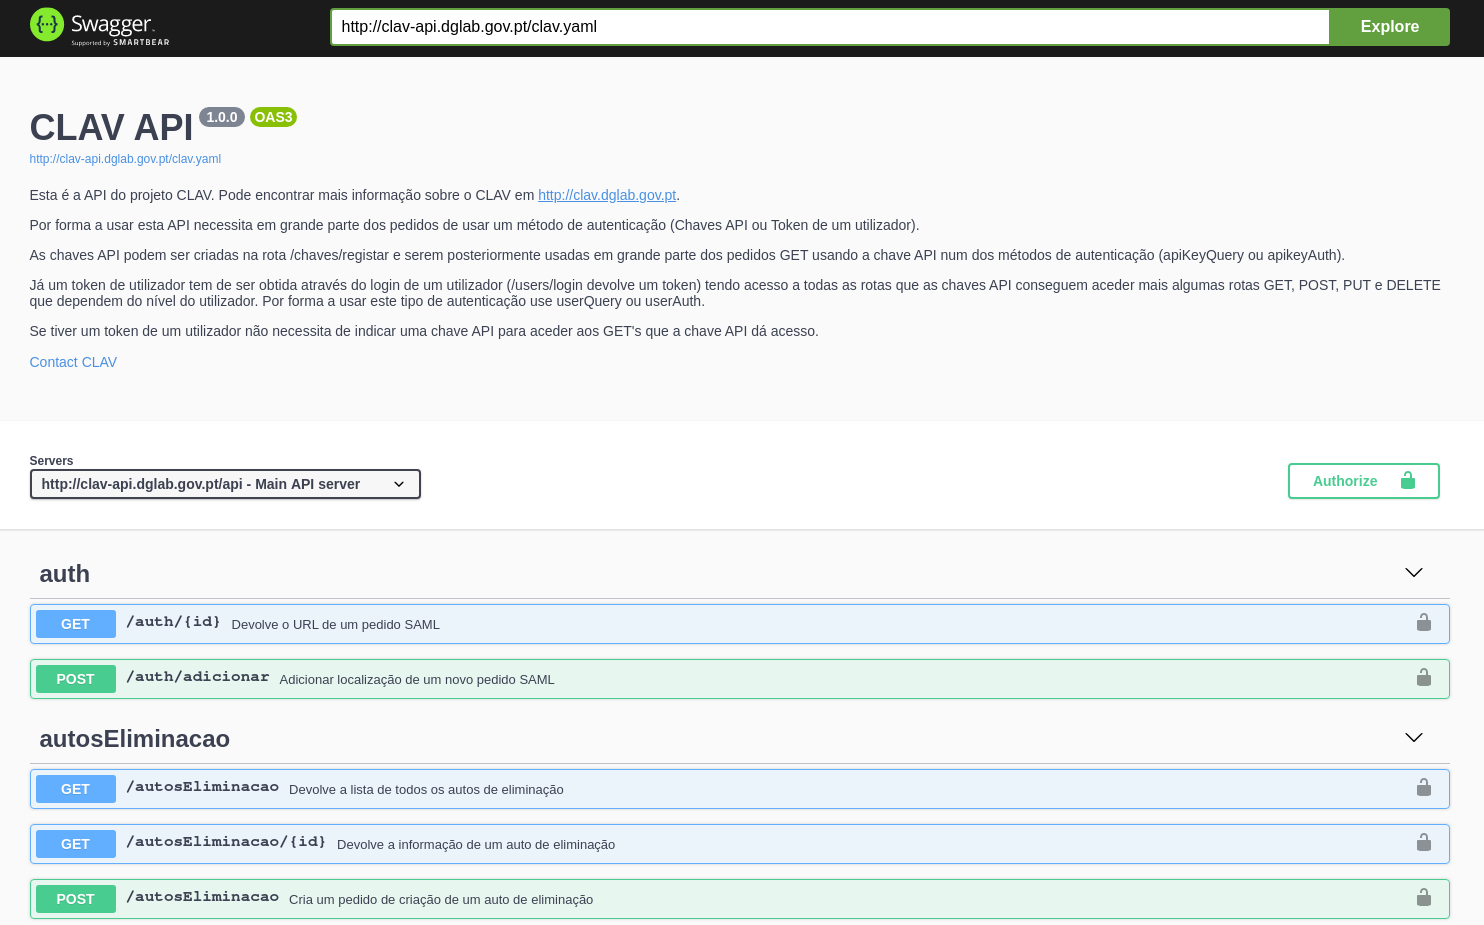
\includegraphics[width=0.7\textwidth]{img/swaggerUI.png}
    \caption{\textit{Swagger \acrshort{ui}} exemplo\label{fig:swaggerUI}}
\end{figure}

\subsubsection{Alternativas}
Existem várias alternativas ao \textit{Swagger \acrshort{ui}}:
\begin{savenotes}
\begin{table}[H]
    \footnotesize
    \centering
    \begin{tabular}{|r|p{0.39\textwidth}|p{0.39\textwidth}|}
    \hline
    Ferramenta & Vantagens & Desvantagens \\ \hline
        \textit{Swagger \acrshort{ui}} &
        \begin{itemize}[leftmargin=0.3cm]
            \setlength\itemsep{0em}
            \item Suporta a especificação \textit{OpenAPI}
            \item \textit{Open-source}
            \item Amplamente usado
        \end{itemize}
        &
        %\begin{itemize}[leftmargin=0.3cm]
        %    \setlength\itemsep{0em}
        %    \item
        %\end{itemize}
        \\ \hline
    \textit{Apiary}\footnote{Ver \url{https://apiary.io/}} &
        \begin{itemize}[leftmargin=0.3cm]
            \setlength\itemsep{0em}
            \item Suporta a especificação \textit{\acrshort{api} Blueprint} e a especificação \textit{OpenAPI}
        \end{itemize}
        &
        \begin{itemize}[leftmargin=0.3cm]
            \setlength\itemsep{0em}
            \item Necessário pagar de forma a puder integrar a documentação da \acrshort{api} num domínio próprio
            \item \textit{Closed-source}
        \end{itemize}
        \\ \hline
    \textit{\acrshort{api} Console}\footnote{Ver \url{https://github.com/mulesoft/api-console}} &
        \begin{itemize}[leftmargin=0.3cm]
            \setlength\itemsep{0em}
            \item Suporta a especificação \acrshort{raml} e a especificação \textit{OpenAPI}
            \item \textit{Open-source}
        \end{itemize}
        &
        %\begin{itemize}[leftmargin=0.3cm]
        %    \setlength\itemsep{0em}
        %    \item
        %\end{itemize}
        \\ \hline
    \textit{Slate}\footnote{Ver \url{https://github.com/slatedocs/slate}} &
        \begin{itemize}[leftmargin=0.3cm]
            \setlength\itemsep{0em}
            \item \textit{Open-source}
            \item \acrshort{api} definida em \textit{Markdown}
        \end{itemize}
        &
        \begin{itemize}[leftmargin=0.3cm]
            \setlength\itemsep{0em}
            \item Não suporta nenhuma especificação
        \end{itemize}
        \\ \hline
    \textit{apiDoc}\footnote{Ver \url{https://apidocjs.com/}} &
        \begin{itemize}[leftmargin=0.3cm]
            \setlength\itemsep{0em}
            \item Documentação criada a partir das anotações nos comentários do código
            \item \textit{Open-source} 
        \end{itemize}
        &
        \begin{itemize}[leftmargin=0.3cm]
            \setlength\itemsep{0em}
            \item Não suporta nenhuma especificação
        \end{itemize}
        \\ \hline
    \textit{ReDoc}\footnote{Ver \url{https://github.com/Redocly/redoc}} &
        \begin{itemize}[leftmargin=0.3cm]
            \setlength\itemsep{0em}
            \item Suporta a especificação \textit{OpenAPI}
            \item \textit{Open-source} 
            \item Fácil de integrar
        \end{itemize}
        &
        %\begin{itemize}[leftmargin=0.3cm]
        %    \setlength\itemsep{0em}
        %    \item
        %\end{itemize}
        \\ \hline
    \end{tabular}
    \caption{Comparação entre ferramentas de \acrshort{api}s}
    \label{table:swaggerUI}
\end{table}
\end{savenotes}

\section{Documentação da \acrshort{api} da \acrshort{clav}}\label{sec:soaDocAPI}

Neste secção são aprofundadas algumas bibliotecas que podem ser usadas para a produção da documentação com a 
especificação \textit{OpenAPI} e o \textit{Swagger \acrshort{ui}}. 

De seguida, são aprofundadas duas \textit{packages} que podem ser usadas para criar documentação 
interativa (integração do \textit{Swagger UI}) para uma \acrshort{api} \acrshort{rest} criada com 
\textit{Node.js} e \textit{Express.js}:~\cite{swaggerNode}
\begin{itemize}
    \item \texttt{swagger-node-express}
    \begin{itemize}
        \item Vantagens
        \begin{itemize}
            \item Módulo oficial suportado pelo \textit{Swagger};
            \item É \textit{open-source} e como tal é possível contribuir para a correção de problemas;
            \item A solução contém \textit{Swagger Editor} e \textit{Swagger Codegen} e como tal tanto 
            podemos usar uma abordagem \textit{top-down} como \textit{bottom-up}.
        \end{itemize}
        \item Desvantagens
        \begin{itemize}
            \item Instalação manual do \textit{Swagger \acrshort{ui}}. O código do \textit{Swagger \acrshort{ui}} 
            tem de ser copiado manualmente para o projeto e sempre que há uma atualização é necessário copiar 
            novamente manualmente;
            \item Instalação complexa. Por forma a aplicação hospedar a documentação é necessário adicionar 
            algumas rotas ao servidor para além das já definidas na especificação \textit{OpenAPI};
            \item Fraca documentação.
        \end{itemize}
    \end{itemize}
    \item \texttt{swagger-ui-express}
    \begin{itemize}
        \item Vantagens
        \begin{itemize}
            \item É \textit{open-source} e como tal é possível contribuir para a correção de problemas;
            \item Não é necessário copiar manualmente o \textit{Swagger \acrshort{ui}};
            \item De fácil instalação, apenas é necessário adicionar uma rota aonde estará hospedada a documentação;
            \item Boa documentação.
        \end{itemize}
        \item Desvantagens
        \begin{itemize}
            \item Não é o módulo oficial suportado pelo \textit{Swagger}.
        \end{itemize}
    \end{itemize}
\end{itemize}

Das duas, a \texttt{swagger-ui-express} é a de mais simples implementação e de mais fácil manutenção.

\begin{lstlisting}[language=javascript, caption=Exemplo de uso do \texttt{swagger-ui-express}, label=exem:suie]
var swaggerUI = require('swagger-ui-express')
//JSON
var swaggerDocument = require('./swagger.json')
//ou YAML
var yaml = require('js-yaml')
var fs = require('fs')
var swaggerDocument = yaml.load(fs.readFileSync('./swagger.yaml'))

app.use('/doc', swaggerUI.serve, swaggerUI.setup(swaggerDocument));
\end{lstlisting}

No exemplo~\ref{exem:suie} a documentação da \acrshort{api} está presente na rota \texttt{'/doc'}. 
Neste exemplo percebe-se como carregar uma especificação \textit{OpenAPI} em \acrshort{json} bem como 
em \acrshort{yaml}. Quanto ao \textit{middleware} \texttt{serve} retorna os ficheiros estáticos necessários 
para hospedar o \textit{Swagger \acrshort{ui}}. Já o segundo \textit{middleware} \texttt{setup} para além de 
poder receber o documento com a especificação \textit{OpenAPI} pode também receber um outro parâmetro de opções 
que o utilizador pode definir para a apresentação interativa da documentação com o 
\textit{Swagger \acrshort{ui}}\footnote{As opções possíveis estão presentes em \url{https://github.com/scottie1984/swagger-ui-express}. Para o atributo (opção) \texttt{swaggerOptions} as opções possíveis estão presentes em \url{https://github.com/swagger-api/swagger-ui/blob/master/docs/usage/configuration.md}}.

Agora há duas abordagens possíveis de realizar a documentação:
\begin{itemize}
    \item Documentação de cada rota nos comentários da rota através da utilização da 
    \textit{package} \texttt{swagger-jsdoc}\footnote{Ver \url{https://github.com/Surnet/swagger-jsdoc}};
    \item Documentação à parte do código.
\end{itemize}

A abordagem da documentação à parte do código permite modularizar a documentação. A modularização da documentação 
pode ser realizada através do uso da \textit{package} \texttt{yaml-include}\footnote{Ver \url{https://github.com/claylo/yaml-include}}. Esta \textit{package} permite que o documento \acrshort{yaml} da especificação \textit{OpenAPI} possa ser dividida por vários ficheiros para além do que já é permitido através do uso de \verb|$ref| da especificação \textit{OpenAPI}. A \textit{package} permite a inclusão de arquivos \acrshort{yaml} externos ou a inclusão de pastas de ficheiros \acrshort{yaml}. Esta funcionalidade é desaprovada pela equipa de desenvolvimento do \acrshort{yaml} contudo ajuda e simplifica a construção do ficheiro de especificação \textit{OpenAPI}.

\begin{lstlisting}[language=yaml, caption=Exemplo de uso do \texttt{yaml-include} no documento de especificação \textit{OpenAPI}(\textit{index.yaml}), label=exem:yamli]
openapi: 3.0.0
info:
  description: Esta é a API do projeto CLAV. Pode encontrar mais informação sobre o CLAV em [http://clav.dglab.gov.pt](http://clav.dglab.gov.pt).
  version: 1.0.0
  title: CLAV API
  contact:
    name: CLAV
    email: clav@dglab.gov.pt
servers:
  - url: http://localhost:7779/api
    description: Local API server
paths: !!inc/dir [ 'paths' ]
components:
  schemas: !!inc/dir [ 'schemas', excludeTopLevelDirSeparator: true ]
  securitySchemes: !!inc/file '/security/schemes.yaml'
\end{lstlisting}

O ficheiro \textit{index.yaml} será a raiz do documento de especificação \textit{OpenAPI} a ser gerado com 
a \textit{package} \texttt{yaml-include}. A seguinte estrutura dos ficheiros exemplifica como se pode dividir a 
documentação por vários ficheiros com esta \textit{package} para gerar o documento de especificação \textit{OpenAPI}:
\begin{lstlisting}[language=pseudocode, caption=Exemplo de estrutura dos ficheiros para gerar o documento de especificação \textit{OpenAPI}, label=exem:faf]
* index.yaml
* paths/
    * classes/
        * get.yaml
        * ~id/
            * get.yaml
    * users/
        * ~id/
            * post.yaml
            * delete.yaml
* schemas/
    * User.yaml
* security/
    * schemes.yaml
\end{lstlisting}

Assim, o \texttt{!!inc/dir} fará com que no ficheiro \textit{index.yaml} na \textit{tag} \textit{paths} sejam 
incluídos todos os ficheiros que estão na pasta \textit{paths}. Cada ficheiro corresponderá a uma determinada 
rota com um determinado método \acrshort{http}. O método \acrshort{http} é definido a partir do nome do ficheiro 
e o caminho da rota é determinado pelo nome das pastas e do aninhamento destas. Quando o nome da pasta é iniciado 
por ``\verb|~|'' no caminho será colocado o nome da pasta sem o til e entre chavetas (``\{\}'') por forma a 
indicar um parâmetro que é colocado no caminho do pedido.

Já no caso do \texttt{!!inc/dir} dos \textit{schemas} a opção \texttt{excludeTopLevelDirSeparator} permite que 
os ficheiros que estejam dentro da pasta \textit{schemas} (mas não aninhados dentro de outras pastas) sejam 
incluídos sem qualquer aninhamento, assumindo o nome do ficheiro como o atributo a colocar.

Existe também o \texttt{!!inc/file} que permite incluir sobe uma determinada \textit{tag} a informação presente 
no ficheiro referenciado pelo caminho.

O documento de especificação \textit{OpenAPI} final gerado será:
\begin{lstlisting}[language=yaml, caption=Documento de especificação \textit{OpenAPI} gerado a partir do ficheiro \textit{index.yaml} com o uso da \textit{package} \texttt{yaml-include}, label=exem:yamlif]
openapi: 3.0.0
info:
  description: Esta é a API do projeto CLAV. Pode encontrar mais informação sobre o CLAV em [http://clav.dglab.gov.pt](http://clav.dglab.gov.pt).
  version: 1.0.0
  title: CLAV API
  contact:
    name: CLAV
    email: clav@dglab.gov.pt
servers:
  - url: http://localhost:7779/api
    description: Local API server
paths:
  /classes:
    get:
      <conteúdo do ficheiro paths/classes/get.yaml>
  /classes/{id}:
    get:
      <conteúdo do ficheiro paths/classes/~id/get.yaml>
  /users/{id}:
    post:
      <conteúdo do ficheiro paths/users/~id/post.yaml>
    delete:
      <conteúdo do ficheiro paths/users/~id/delete.yaml>
components:
  schemas:
    User:
      <conteúdo do ficheiro schemas/User.yaml>
  securitySchemes:
    <conteúdo do ficheiro security/schemes.yaml>
\end{lstlisting}

No final teremos um ficheiro no formato \acrshort{yaml} com toda a documentação da \acrshort{api} que puderá 
então ser usado para alimentar a documentação dinâmica \textit{Swagger \acrshort{ui}}.

\section{Exportação de dados}\label{sec:exportacao}

Esta tese tem como um dos objetivos a exportação de dados da \acrshort{api} de Classes (\acrshort{lc}), Entidades, Tipologias e Legislações em formato \acrshort{json}, \acrshort{xml} e \acrshort{csv}. Além disso, deve permitir a exportação da ontologia (possuidor da informação das variantes referidas a exportar) nos formatos \acrshort{rdf} seguintes: \acrshort{turtle}, \acrshort{json-ld} e \acrshort{rdf}/\acrshort{xml}.

A \acrshort{api} de dados já devolve a sua informação em \acrshort{json}. Portanto, por forma a realizar a exportação dos dados para outros formatos é necessário realizar a conversão de \acrshort{json} para o formato de saída pretendido. Como tal, nesta secção será aprofundada algumas bibliotecas disponíveis no \acrshort{npm} que têm como objetivo exportar de \acrshort{json} para \acrshort{xml} ou de \acrshort{json} para \acrshort{csv}. É por fim, investigado como poderá ser exportada a ontologia a partir do GraphDB.

\subsection{\acrshort{xml}}

Comecemos por perceber o que é o \acrfull{xml}. Como se pode perceber pelo nome o \acrshort{xml} é uma linguagem \textit{Markup}, ou seja, uma linguagem que anota o texto para que a máquina possa manipular o texto de acordo com as anotações. O \acrshort{xml} foi desenhado para ser de fácil leitura tanto para humanos como para máquinas e tem como principal intuito o armazenamento e transporte de informação (o tal texto anotado). Além disso é extensível visto que permite que criemos as nossas \textit{tags}.

\begin{lstlisting}[language=xml, caption=Pequeno exemplo em \acrshort{xml}, label=exem:xmlEx]
<?xml version = "1.0" encoding = "UTF-8"?>
<pessoa>
    <nome>Maria</nome>
    <idade tipo="numero">23</idade>
    <morada>
        <pais>Portugal</pais>
        <cidade>Braga</cidade>
    </morada>
    <altura unidade="cm">160</altura>
    <!--Isto é um comentário-->
</pessoa>
\end{lstlisting}

De seguida serão apresentadas, de forma simplificada, as regras de sintaxe aplicadas ao \acrshort{xml} para cada componente deste.

\begin{itemize}
    \item \textbf{Declaração \acrshort{xml}} \\
    \verb|<?xml version = "1.0" encoding = "UTF-8"?>| \\
    Opcional, especifica a versão do \acrshort{xml} e o \textit{encoding} usado no documento
    \begin{itemize}
        \item A declaração é \textit{case-sensitive} pelo que deve começar obrigatoriamente por \texttt{xml}
        \item Se presente no documento, a declaração tem de ser obrigatoriamente o primeiro componente
    \end{itemize}
    \item \textbf{\textit{Tags} e elementos} \\
    \verb|<nome>Maria</nome>| ou \verb|<semnome/>|
    \begin{itemize}
        \item Cada elemento tem de ser fechado seja por uma \textit{tag} (\textit{tag} final), ou como apresentado acima pela própria \textit{tag}.
        \item Os elementos \acrshort{xml} podem conter elementos filhos mas estes não se podem sobrepor, ou seja, uma \textit{tag} final de um elemento tem de ter o mesmo nome que a última \textit{tag} inicial ainda sem \textit{tag} final. 
        \item Um documento \acrshort{xml} apenas pode ter um elemento na raiz do documento (elemento \textit{root})
        \item Os nomes das \textit{tags} são \textit{case-sensitive}, portanto, a \textit{tag} inicial e final de um elemento têm de ser exatamente iguais
    \end{itemize}
    \item \textbf{Atributos} \\
    \verb|<altura unidade="cm">160</altura>| \\
    onde `unidade' é o nome do atributo e `cm' é o valor do atributo. Um atributo especifica uma propriedade de um elemento
    \begin{itemize}
        \item Um elemento pode ter zero, um ou mais atributos
        \item Os nomes dos atributos são \textit{case-sensitive}
        \item Um atributo não pode ter dois valores num elemento, ou seja, não pode ser declarado duas ou mais vezes num mesmo elemento
        \item Os nomes dos atributos não podem possuir aspas, mas os valores tem de ser encapsulados por aspas
    \end{itemize}
    \item \textbf{Referências \acrshort{xml}} \\
    \verb|&amp;| ou \verb|&#65| \\
    Há dois tipos de referências, Referências Entidade ou Referências Caractere. A primeira existe por forma a serem representadas por estas referências os caracteres não permitidos no texto anotado visto representarem parte da sintaxe do \acrshort{xml}.
    \begin{center}
        \begin{tabular}{|c|c|}
            \hline
            Caractere não permitido & Entidade \\ \hline
            < & \&lt; \\ \hline
            > & \&gt; \\ \hline
            \& & \&amp; \\ \hline
            ' & \&apos; \\ \hline
            " & \&quot; \\ \hline
        \end{tabular}
    \end{center}
    O segundo tipo de referências tem o mesmo intuito mas permite que seja representado qualquer caractere representável em \textit{Unicode}. O número que se segue ao \textit{hashtag} é referente ao código decimal em \textit{Unicode}. Assim \verb|&#65| representa o caractere `A'.
    \item \textbf{Texto anotado} \\
    Espaços em branco, \textit{tabs}, ou novas linhas, são ignoradas quando presentes entre elementos e entre atributos. Como já referido há caracteres reservados pelo que se pretende usá-los no texto anotado deve trocar esses caracteres pelas suas referências.
\end{itemize}

\subsubsection{Bibliotecas de conversão}

Nesta secção serão abordadas algumas bibliotecas de conversão de \acrshort{json} para \acrshort{xml}, aquelas com maior popularidade e adesão no \acrshort{npm}.

Por forma a ter uma ideia do resultado devolvido por cada biblioteca será usado o seguinte exemplo:
\begin{lstlisting}[language=json, caption=Exemplo em \acrshort{json} a converter, label=exem:jsonBib]
[
    {
        "nome": "Maria",
        "idade": "22",
        "morada": {
            "pais": "Portugal",
            "cidade": "Braga"
        }
    },
    {
        "nome": "João",
        "idade": "24",
        "morada": {
            "pais": "Portugal",
            "cidade": "Vila Real"
        }
    }
]
\end{lstlisting}

\paragraph{\href{https://www.npmjs.com/package/xml-js}{\texttt{xml-js}}} \mbox{} \\

Esta biblioteca permite a conversão nos dois sentidos, ou seja, de \acrshort{json} para \acrshort{xml} e de \acrshort{xml} para \acrshort{json}.

As principais características que esta biblioteca possui para uma conversão de \acrshort{json} para \acrshort{xml} são:
\begin{itemize}
    \item Mantém a ordem dos elementos
    \item Totalmente compatível com \acrshort{xml}
    \item Reversível, é possível reverter o resultado para o original
    \item Podem ser fornecidas funções personalizadas para processamento adicional para diferentes partes do \acrshort{xml} ou do \acrshort{json} a converter
\end{itemize}

\begin{lstlisting}[language=xml, caption=Resultado da conversão do exemplo~\ref{exem:jsonBib} usando o conversor \texttt{xml-js}]
<0>
    <nome>Maria</nome>
    <idade>22</idade>
    <morada>
        <pais>Portugal</pais>
        <cidade>Braga</cidade>
    </morada>
</0>
<1>
    <nome>João</nome>
    <idade>24</idade>
    <morada>
        <pais>Portugal</pais>
        <cidade>Vila Real</cidade>
    </morada>
</1>
\end{lstlisting}

\paragraph{\href{https://www.npmjs.com/package/xmlbuilder}{\texttt{xmlbuilder}}} \mbox{} \\

A biblioteca tem como intuito principal a construção de documentos \acrshort{xml} através do uso de funções, como se pode comprovar de seguida:

\begin{lstlisting}[language=javascript, caption=Código para a construção em \acrshort{xml} do exemplo~\ref{exem:xmlEx} usando o \texttt{xmlbuilder}]
var builder = require('xmlbuilder');
 
var xml = builder.create('pessoa')
    .ele('nome', 'Maria')
    .up()
    .ele('idade', {'tipo': 'numero'}, '23')
    .up()
    .ele('morada')
    .ele('pais', 'Portugal')
    .up()
    .ele('cidade', 'Braga')
    .up()
    .up()
    .ele('altura', {'unidade': 'cm'}, '160')
    .up()
    .com('Isto é um comentário')
    .end({ pretty: true});
\end{lstlisting}

Além disso, permite a geração do \acrshort{xml} a partir de um objeto \acrshort{json} o que permite, como tal, a conversão de \acrshort{json} para \acrshort{xml} que se necessita.

\begin{lstlisting}[language=xml, caption=Resultado da conversão do exemplo~\ref{exem:jsonBib} usando o conversor \texttt{xmlbuilder}]
<?xml version="1.0" encoding="utf-8"?>
<nome>Maria</nome>
<idade>22</idade>
<morada>
  <pais>Portugal</pais>
  <cidade>Braga</cidade>
</morada>
<nome>João</nome>
<idade>24</idade>
<morada>
  <pais>Portugal</pais>
  <cidade>Vila Real</cidade>
</morada>
\end{lstlisting}

Na construção do documento a partir de um objecto, quando se pretende que um elemento tenha um atributo, é necessário que o objeto para essa chave possua um objeto em vez de apenas o valor. Nesse objeto, as propriedades começadas por `@' indicam atributos (\verb|'@unidade':'cm'| onde `unidade' é o nome do atributo e `cm' é o valor do atributo) e a propriedade '\#text' representa o valor do elemento.

Há também a possibilidade de sobrescrever as funções usadas para escrever o documento \acrshort{xml} (funções de escrita dos elementos, comentários, etc) bem como as funções que convertem os valores (texto anotado, nome de elementos e atributos, etc).

Por fim, convém referir que esta biblioteca já possui uma sucessora, \href{https://www.npmjs.com/package/xmlbuilder2}{\texttt{xmlbuilder2}}, que foi redesenhada por forma a estar em total conformidade com a especificação moderna do \acrshort{dom}.

\paragraph{\href{https://www.npmjs.com/package/xml2js}{\texttt{xml2js}}} \mbox{} \\

De igual forma como a biblioteca \texttt{xml-js}, esta biblioteca consegue converter de \acrshort{json} para \acrshort{xml} como de \acrshort{xml} para \acrshort{json}. 

\begin{lstlisting}[language=xml, caption=Resultado da conversão do exemplo~\ref{exem:jsonBib} usando o conversor \texttt{xml2js}]
<?xml version="1.0" encoding="UTF-8" standalone="yes"?>
<root>
  <nome>Maria</nome>
  <idade>22</idade>
  <morada>
    <pais>Portugal</pais>
    <cidade>Braga</cidade>
  </morada>
  <nome>João</nome>
  <idade>24</idade>
  <morada>
    <pais>Portugal</pais>
    <cidade>Vila Real</cidade>
  </morada>
</root>
\end{lstlisting}

Se se pretende que um determinado elemento possua atributos é necessário que o objeto para esse elemento seja um objeto (\verb|{$: {unidade: 'cm'}, _: '160'}|) onde `\_' é o texto anotado e os vários atributos devem estar no objeto da propriedade `\$' em que o nome da propriedade é o nome do atributo e o valor da propriedade e o valor do atributo.

\subsection{\acrshort{csv}}

\acrfull{csv} como o seu acrónimo indica é um documento em que os campos de um registo são separados por uma vírgula. Contudo, os campos não precisam de ser obrigatoriamente separados por vírgula já que podem também ser separados por ponto e vírgula, \textit{tabs}, \textit{pipes} (`|') ou ainda outro qualquer caractere que se pretenda usar. Quando se usa o caractere separador ou uma nova linha (`\backslash{}n') no campo de um registo, por forma a não ser considerado como um separador de campos ou de registos respetivamente, pode-se encapsular os valores por aspas (`"') sendo que também se pode usar outro caractere em vez das aspas. Já quando se usa o caractere de encapsulamento no campo de um registo este deve ser protegido (\texttt{escaped}) repetindo o mesmo caractere de encapsulamento.

Um documento \acrshort{csv} é nada mais que uma tabela que guarda dados em texto. É usado essencialmente para a troca de dados.

Após esta pequena introdução ao \acrshort{csv} apresenta-se as regras de sintaxe para a criação de um documento \acrshort{csv}:
\begin{itemize}
    \item Campos separados com um separador, normalmente uma vírgula
    \item Cada registo deve estar numa linha. Cada registo deve começar numa linha, mas cada registo pode ter várias linhas, desde que os campos multi linha sejam encapsulados por aspas
    \item Após o último registo não deve estar presente um \textit{carriage return}
    \item Opcionalmente, na primeira linha do documento, deve estar presente o cabeçalho com os nomes das colunas separados pelo separador usado no resto do documento
    \item O caractere de encapsulamento deve ser usado para encapsular um campo quando necessário (pode ser usado sempre), isto é, quando o caractere separador ou uma nova linha (`\backslash{}n') são usados num campo de um registo
\end{itemize}

\begin{lstlisting}[caption=Pequeno exemplo em \acrshort{csv}, label=exem:csvEx]
Nome,Idade,País,Cidade,Altura
"Silva, Maria",23,Portugal,Braga,160cm
\end{lstlisting}

\subsubsection{Bibliotecas de conversão}

Nesta secção irá também ser aprofundada algumas bibliotecas de conversão de \acrshort{json} para \acrshort{csv}, aquelas com maior popularidade no \acrshort{npm}.

\paragraph{\href{https://www.npmjs.com/package/papaparse}{\texttt{papaparse}}} \mbox{} \\

O \texttt{papaparse} tem como principal objetivo realizar o \textit{parse} de ficheiros \acrshort{csv}. Consegue contudo reverter, convertendo de \acrshort{json} para \acrshort{csv}.

\begin{lstlisting}[caption=Resultado da conversão do exemplo~\ref{exem:jsonBib} usando o conversor \texttt{papaparse}, label=exem:papaparse]
nome,idade,morada
Maria,22,[object Object]
João,24,[object Object]
\end{lstlisting}

Olhando para o resultado~\ref{exem:papaparse} consegue-se perceber que o conversor não consegue converter objetos aninhados. Para além disso, apesar de haver a possibilidade de alterar o caractere separador, o caractere de \textit{escape}, o caractere de nova linha bem como definir o nome das colunas no cabeçalho, não é possível definir uma função por forma a alterar a conversão dos campos de cada propriedade.

\paragraph{\href{https://www.npmjs.com/package/json2csv}{\texttt{json2csv}}} \mbox{} \\

Biblioteca totalmente dedicada à conversão de \acrshort{json} para \acrshort{csv}. Tem como principais características:
\begin{itemize}
    \item Permite a alteração dos caracteres de separação, de encapsulamento e de nova linha
    \item \textit{Escape} automático
    \item Permite escolher que campos devolver (mesmo em objetos aninhados ou listas aninhadas) e que cabeçalho associar a cada campo
    \item Aceita funções de transformação para cada campo
\end{itemize}

\begin{lstlisting}[caption=Resultado da conversão do exemplo~\ref{exem:jsonBib} usando o conversor \texttt{json2csv}, label=exem:json2csv]
"nome","idade","morada.pais","morada.cidade"
"Maria","22","Portugal","Braga"
"João","24","Portugal","Vila Real"
\end{lstlisting}

Para além disso permite o \textit{unwind} de uma propriedade que possua uma lista, fazendo com que sejam gerados x registos de acordo com o tamanho da lista, sendo alterado apenas os valores que provêm da lista. Infelizmente isto acrescenta mais colunas, não permitindo que no caso de os elementos da lista (filhos) tenham a mesma estrutura que o pai, sejam adicionados como novos registos, sem adicionar novas colunas e sem repetir a informação do pai. 

Por exemplo, se pretendermos converter o seguinte documento \acrshort{json}:
\begin{lstlisting}[language=json, caption=Outro exemplo em \acrshort{json} a converter, label=exem:jsonBib2]
[
    {
        "nome": "Maria",
        "idade": "22",
        "morada": {
            "pais": "Portugal",
            "cidade": "Braga"
        },
        "filhos": [
          {
            "nome": "António",
            "idade": "24",
            "morada": {
                "pais": "Portugal",
                "cidade": "Aveiro"
            }
          }
        ]
    },
    {
        "nome": "João",
        "idade": "24",
        "morada": {
            "pais": "Portugal",
            "cidade": "Vila Real"
        },
        "filhos": []
    }
]
\end{lstlisting}

Usando este conversor é possível obter:
\begin{lstlisting}[caption=Resultado da conversão do exemplo~\ref{exem:jsonBib2} usando o conversor \texttt{json2csv}]
"nome","idade","morada.pais","morada.cidade","filhos.nome","filhos.idade","filhos.morada.pais","filhos.morada.cidade"
"Maria","22","Portugal","Braga","António","2","Portugal","Braga"
"João","24","Portugal","Vila Real",,,,
\end{lstlisting}

Quando o resultado pretendido seria por exemplo:
\begin{lstlisting}[caption=Resultado pretendido da conversão do exemplo~\ref{exem:jsonBib2}]
"nome","idade","morada.pais","morada.cidade"
"Maria","22","Portugal","Braga",
"António","24","Portugal","Aveiro"
"João","24","Portugal","Vila Real"
\end{lstlisting}

\subsection{Ontologia}

\subsubsection{O que é uma ontologia?}

Uma ontologia é uma descrição formal e explícita de conceitos num domínio de discurso (classes, chamado às vezes de conceitos), propriedades de cada conceito que descrevem várias características e atributos do conceito (\textit{slots}, às vezes chamados de funções ou propriedades) e restrições sobre \textit{slots} (facetas, às vezes chamadas de restrições de função).~\cite{ontologyProt} Uma ontologia, juntamente com um conjunto de instâncias individuais de classes, constitui uma base de conhecimento.~\cite{ontologyProt}

Uma ontologia pode ser dividida em duas partes:
\begin{itemize}
    \item Estrutura: Onde é definido as classes, as propriedades (\textit{slots}) e as restrições das propriedades (facetas)
    \item População: Onde é definido indivíduos (de classes) e propriedades dos indivíduos. Esta parte é construída tendo por base a estrutura definida.
\end{itemize}
De certa forma, a estrutura é como se fosse o modelo definido e a população a informação guardada respeitando o modelo definido.

Falemos agora um pouco mais sobre cada componente de uma ontologia.

Começando pelas classes, estas correspondem a conceitos, sendo que uma classe pode ter subclasses (onde uma subclasse herda as propriedades da sua superclasse) e superclasses. Para além disso, as classes possuem instâncias (ou indivíduos). Quanto às propriedades das classes existem dois tipos:
\begin{itemize}
    \item Atributos: propriedade que permite definir uma característica de uma classe (ou indivíduo) (p.e: Se pessoa for uma classe, o nome será um atributo)
    \item Relações: propriedade que permite estabelecer relações entre classes (ou indivíduos) (p.e: A relação de pai entre duas pessoas) 
\end{itemize}

As próprias propriedades podem ser caracterizadas através das restrições. As principais restrições são:
\begin{itemize}
    \item Cardinalidade: Indica quantos valores pode ter uma propriedade, \texttt{0} a \texttt{n} (p.e: Uma pessoa só tem um pai biológico.; outro exemplo: Uma pessoa pode ter várias nacionalidades)
    \item Tipo de valor: Indica que tipo de valor terá a propriedade (atributo), \textit{string}, número, \textit{boolean}, etc (p.e: A idade de uma pessoa é um número; outro exemplo: O nome de uma pessoa é uma \textit{string})
    \item \textit{Domain} e \textit{Range}: Indica que tipo de instâncias podem ser relacionadas por uma propriedade. O \textit{Domain} indica a quem pertence a propriedade (atributo ou relação). Já o \textit{Range} indica para uma relação o tipo de instâncias que podem ser relacionadas com o \textit{Domain} (p.e: Na relação pai, o seu \textit{Domain} e o seu \textit{Range} são iguais a Pessoa.; outro exemplo: Seja Animal outra classe, a relação tem dono tem como \textit{Domain} Animal e como \textit{Range} Pessoa; ainda outro exemplo: O \textit{Domain} do atributo nome é Pessoa)
\end{itemize}

\subsubsection{\textit{Web} Semântica}

A \textit{web} semântica é uma extensão da \acrshort{www} com o objetivo de tornar a informação da internet legível por máquinas (\textit{machine-readable}).

Para isso a \acrfull{w3c} está a ajudar a criar a \textit{stack} tecnológica necessária. O termo \textit{web} semântica é a visão da \acrshort{w3c} acerca da \textit{Linked Data} na \textit{Web}, ou seja, é a web dos dados em que a coleção de tecnologias da \textit{web} semântica (\acrshort{rdf}, \acrshort{sparql}, \acrshort{owl}, \acrshort{skos}, etc) oferece um ambiente onde as pessoas podem criar bases de dados na \textit{web}, construir ontologias e escrever regras para manipular os dados; e onde as aplicações podem questionar esses dados e desenhar inferências usando vocabulários.

Para tornar a \textit{web} dos dados uma realidade é necessário existir uma grande quantidade de dados na \textit{web} num formato \textit{standard} (\acrshort{rdf}), acessível e gerível pelas ferramentas da \textit{web} semântica. Além disso, a \textit{web} semântica necessita também que existam relações entre os dados para criar a \textit{web} dos dados (\textit{Linked Data}). É também importante ser possível configurar \textit{query endpoints} para aceder aos dados mais convenientemente. A \acrshort{w3c} fornece uma palete de tecnologias, das quais se destaca o \acrshort{sparql}, para obter acesso aos dados.

A \textit{Linked Data} é usada para a integração em grande escala e o \textit{reasoning}\footnote{Em \textit{web} semântica é a inferência de informação (triplos) a partir de um conjunto de factos (triplos), ou seja, a descoberta de novos factos (triplos)} dos dados na \textit{web}.

Na \textit{web} semântica, os vocabulários definem os conceitos e os relacionamentos usados para descrever e representar uma área de interesse. Não há uma divisão clara entre o que é referido como ``vocabulários'' e ``ontologias''. A tendência é usar a palavra ``ontologia'' para coleções de termos mais complexos e mais formais, enquanto que ``vocabulário'' nas coleções menos formais. A \acrshort{w3c} oferece várias técnicas para descrever e definir diferentes formas de vocabulários num formato \textit{standard}. Estas incluem \acrshort{rdf} e \acrshort{rdf} Schemas, \acrshort{skos}, \acrshort{owl} e \acrshort{rif}. A escolha da tecnologia depende da complexidade e do rigor necessário.

Tal como as bases de dados relacionais ou o \acrshort{xml} necessitam de linguagens de pesquisa (\textit{query}) específicas (\acrshort{sql} e \textit{XQuery}, respetivamente), a \textit{web} dos dados, tipicamente representada usado \acrshort{rdf} como formato de dados, necessita também de uma linguagem de pesquisa. Isto é providenciado pelo \acrshort{sparql}, que é também um protocolo de comunicação, permitindo enviar \textit{queries} e receber resultados, por exemplo, através de \acrshort{http} ou \acrshort{soap}.

As \textit{queries} \acrshort{sparql} são baseadas em padrões (triplos). O \acrshort{rdf} pode ser visto como um conjunto de relacionamentos entre recursos (triplos \acrshort{rdf}). As \textit{queries} \acrshort{sparql} possuem um ou mais padrões semelhantes aos triplos \acrshort{rdf}, exceto que um ou mais dos recursos constituintes referenciados são variáveis. Um motor \acrshort{sparql} retornará os recursos que para todos os triplos correspondem a esses padrões. A informação devolvida pelos \textit{endpoints} \acrshort{sparql} pode ser uma tabela ou por exemplo \acrshort{json}.

\subsubsection{\textit{GraphDB}}

O \textit{GraphDB} é uma \acrfull{bd} Semântica baseada em grafos compatível com os padrões \acrshort{w3c}. É a base de dados principal quando se pretende trabalhar com a \textit{web} semântica. Suporta \acrshort{rdf} e \acrshort{sparql} e possui funcionalidades de exportação dos triplos presentes numa \acrshort{bd} armazenada no \textit{GraphDB}.

Para um fácil uso e compatibilidade com os \textit{standards} da indústria, o \textit{GraphDB} implementou as interfaces da \textit{framework} \textit{RDF4J}, a especificação do protocolo \acrshort{w3c} \acrshort{sparql}\footnote{Ver \url{https://www.w3.org/TR/sparql11-protocol/}} e suporta vários formatos de serialização \acrshort{rdf}\footnote{\label{fnRDF}\textit{TriG}, \textit{BinaryRDF}, \textit{TriX}, \textit{N-Triples}, \textit{N-Quads}, \acrshort{n3}, \acrshort{rdf}/\acrshort{xml}, \acrshort{rdf}/\acrshort{json}, \acrshort{json-ld} e \acrshort{turtle}}.~\cite{graphdbAbout}

O \textit{GraphDB} é um \textit{plugin} \acrshort{sail} para a \textit{framework} \textit{RDF4J} fazendo uso extensivo dos recursos e infraestrutura do \textit{RDF4J} especialmente do modelo \acrshort{rdf}, dos \textit{parsers} \acrshort{rdf} e dos motores de pesquisa.~\cite{graphdbArch}

Assim, o \textit{GraphDB} possui uma \acrshort{rest} \acrshort{api} do servidor \textit{RDF4J}\footnote{Ver \url{https://rdf4j.org/documentation/rest-api/}} a partir da qual é possível obter todos os triplos de uma \acrshort{bd} através da rota
\begin{verbatim}
<url do GraphDB>/repositories/<id do repositório (BD)>/statements
\end{verbatim}
indicando no cabeçalho \acrshort{http} \textit{Accept} o formato de serialização \acrshort{rdf}\footnoteref{fnRDF} de saída (\textit{\acrshort{mime} type}\footnote{\textit{Standard} que indica a natureza e o formato de um documento, ficheiro ou conjunto de \textit{bytes}. Ver \href{https://tools.ietf.org/html/rfc6838}{RFC 6838}}) dos triplos.

\section{Let's Encrypt}

Para ativar o \acrshort{https} num website ou numa \acrshort{api}, ou seja num domínio, é necessário um \acrfull{ca} de onde obter os certificados.

Para o caso da \acrshort{clav} necessita-se de um \acrshort{ca} gratuito e onde seja possível gerar certificados \acrfull{dv} (garantem apenas a validade do domínio e da informação trocada entre utilizador e domínio~\cite{certsTypes}).

Assim, a escolha recaiu no \textit{Let's Encrypt}, um dos \acrshort{ca}'s mais populares. O \textit{Let's Encrypt} foi criado pela \textit{Linux Foundation} é gratuito e \textit{open-source}. Além disso, tem como patrocinadores/doadores empresas como a \textit{Mozilla}, a \textit{Cisco}, o \textit{Google Chrome}, o \textit{Facebook}, entre outros. 

Para gerar/renovar o certificado \acrshort{dv} é necessário demonstrar que se possui o controlo sobre o domínio. Com o \textit{Let's Encrypt} isto é efetuado através do uso do protocolo \acrfull{acme} que necessita que se corra um agente de gestão de certificados (cliente \acrshort{acme}) no servidor do domínio a gerar o certificado. Assim é possível gerar/renovar certificados automaticamente sem a intervenção humana. Esta automatização é importante porque os certificados do \textit{Let's Encrypt} têm apenas a validade de 3 meses pelo que, se fosse necessário fazer manualmente teria de ser feito pelo menos de 3 em 3 meses.

A escolha do cliente \acrshort{acme} a usar irá depender se se tem acesso à \textit{shell} da máquina do servidor. Em caso afirmativo o \textit{Let's Encrypt} recomenda o uso do cliente \textit{Certbot}~\cite{letEnc}.

Caso não se tenha acesso à \textit{shell} irá depender se o provedor de \textit{hosting} suporta o \textit{Let's Encrypt} ou não. Se suportar então é fácil obter o certificado através do provedor. Caso contrário, pode-se pedir ao provedor o suporte (que não resolve de imediato o problema nem é de resolução garantida) ou se o provedor permitir o \textit{uploud} de certificados é possível através do \textit{Certbot} gerar um certificado em modo manual mas que acarreta efetuar esta tarefa pelo menos de 3 em 3 meses para renovar o certificado pelo que não é recomendado.

Uma pequena chamada de atenção, o \textit{Let's Encrypt} possui \textit{Rate Limits}~\cite{LErateLimits} pelo que num ambiente de testes deve ser usado o ambiente de testes do \textit{Let's Encrypt}\footnote{Ver \url{https://letsencrypt.org/docs/staging-environment/}} e não o de produção.

\subsection{Validação do Domínio}\label{sec:valDom}

Nesta secção será explicado como é realizada a validação do domínio para a geração/renovação/revogação dos certificados.

Na primeira vez que o agente (cliente \acrshort{acme}) interage com o \textit{Let's Encrypt} gera um novo par de chaves e prova ao \textit{Let's Encrypt} que o servidor controla um ou mais domínios.~\cite{domainValidation}

Para iniciar o processo de validação, o cliente \acrshort{acme} questiona o \textit{Let's Encrypt} para que lhe indique o que necessita fazer para provar que controla o domínio~\cite{domainValidation}. Assuma-se que queremos validar o domínio \texttt{example.com}.
O \textit{Let's Encrypt} irá gerar um ou mais conjuntos de desafios após olhar para o nome do domínio.

Há duas formas (desafios) do cliente \acrshort{acme} provar que controla o domínio perante o \textit{Let's Encrypt}~\cite{domainValidation}:
\begin{itemize}
    \item Providenciar um \acrshort{dns} \textit{record} sobre \texttt{example.com}
    \item Providenciar um recurso \acrshort{http} num \acrshort{uri} conhecido em \texttt{http://example.com/} (é colocado normalmente em \texttt{http://example.com/.well-known/acme-challenge})
\end{itemize}

Juntamente com os desafios, o \textit{Let's Encrypt} envia um \textit{nonce} (\textit{string} usada uma única vez) que o cliente deve assinar com a chave privada por forma a garantir que este controla o par de chaves evitando \textit{replay attacks}\footnote{Para mais informação ver \url{https://www.kaspersky.com/resource-center/definitions/replay-attack}}.

Veja-se agora, na figura~\ref{fig:domainValidation}, um exemplo concreto em que o cliente \acrshort{acme} usa o segundo desafio para provar que controla o domínio (\texttt{example.com}):

\begin{figure}[H]
    \centering
    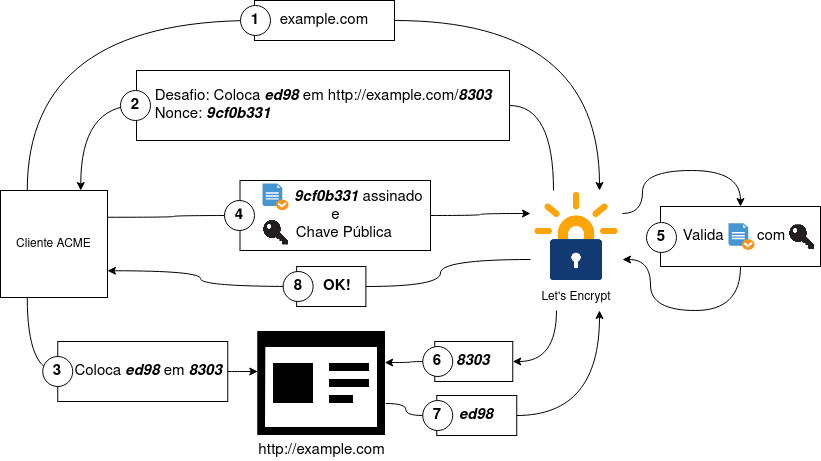
\includegraphics[width=1\textwidth]{img/domainValidation.png}
    \caption{Exemplo de validação do domínio pelo \textit{Let's Encrypt} com sucesso\label{fig:domainValidation}}
\end{figure}

Como o desafio teve sucesso e o \textit{nonce} assinado pelo cliente \acrshort{acme} é válido então o cliente \acrshort{acme} identificado pela chave pública está autorizado a gerir os certificados para o domínio \texttt{example.com}. Assim, para gerar/renovar/revogar o certificado para o domínio basta enviar mensagens de gestão do certificado assinadas com o chave privada (a que assinou o \textit{nonce}) para o \textit{Let's Encrypt}.

\subsection{Cliente \textit{acme.sh}}\label{sec:soaACMEsh}
Apesar do cliente recomendado pelo \textit{Let's Encrypt} ser o \textit{Certbot} este necessita de ter permissões \textit{root} bem como tem várias dependências para ser executado. Já o cliente \textit{acme.sh}\footnote{Ver \url{https://github.com/acmesh-official/acme.sh}} é uma \textit{script} \textit{bash} que para a sua instalação basta efetuar \textit{download} da \textit{script} deste. Além disso, não necessita de quaisquer dependências nem de acesso \textit{root} (apenas necessita em casos especiais). A sua utilização, tal como o \textit{Certbot}, é feita através da execução de comandos \textit{bash}.

Para instalar basta:
\begin{verbatim}
curl https://get.acme.sh | sh
#ou
wget -O -  https://get.acme.sh | sh
\end{verbatim}

Esta instalação irá ativar desde logo a auto renovação dos certificados através da criação de um \textit{cron job}\footnote{Mais informação em \url{https://www.ostechnix.com/a-beginners-guide-to-cron-jobs/}} pelo que o cliente \textit{acme.sh} irá correr periodicamente para verificar e renovar os certificados se necessário.

Para obter um certificado executa-se:
\begin{verbatim}
acme.sh --issue -d <dominio> -w <pasta web root>
\end{verbatim}

Após obter o certificado, este pode ser instalado no \textit{Nginx} com:
\begin{verbatim}
acme.sh --install-cert -d example.com \
    --key-file /path/to/keyfile/in/nginx/key.pem  \
    --fullchain-file /path/to/fullchain/nginx/fullchain.pem \
    --reloadcmd "nginx -s reload"
\end{verbatim}

Neste último comando, o ficheiro de configuração do \textit{Nginx} tem de estar à espera que os ficheiros do certificado estejam em \path{/path/to/keyfile/in/nginx/key.pem} e em \path{/path/to/fullchain/nginx/fullchain.pem}.

\section{\acrshort{api} Gateway}\label{sec:api_gateway}

Uma \textit{\acrshort{api} Gateway} encapsula a arquitetura interna em microserviços de uma aplicação, expondo uma única e simples \acrshort{api} através de um único \acrshort{url}, ou seja, um único ponto de entrada para a aplicação. Em arquiteturas baseadas em microserviços o não uso de uma \textit{\acrshort{api} Gateway} implica que os utilizadores da aplicação tenham provavelmente de agregar dados de diferentes serviços, manter vários \textit{endpoints}, realizar uma maior quantidade de pedidos e ter possivelmente uma autenticação diferente para cada serviço.

Uma \textit{\acrshort{api} Gateway} inclui normalmente~\cite{apiGatInfo,apiGatInfo2}:
\begin{itemize}
    \item Segurança (Autenticação e Autorização)
    \item Gestão de cotas e \textit{throttling}
    \item \textit{Caching}
    \item Processamento e composição da \acrshort{api}
    \item Roteamento
    \item Monitorização da \acrshort{api}
    \item Versionamento (possível automatização)
    \item Balanceamento de carga
    \item \textit{Rate Limit}
\end{itemize}

Além disso, a \textit{\acrshort{api} Gateway} tem como vantagens:~\cite{apiGatInfo, apiGatInfo3}
\begin{itemize}
    \item Simplifica o código da \acrshort{api}
    \item Oferece uma vista única e central da \acrshort{api} e, portanto, é mais provável que permita uma política consistente
    \item A agregação e transformação de dados simplifica a interação dos clientes com os microserviços distribuídos. A agregação de dados permite também reduzir o número de pedidos
    \item Esconde a arquitetura interna e distribui as aplicações baseadas em microserviços reduzindo, geralmente a sobrecarga de configuração 
    \item Código do cliente mais simples e limpo: quando os serviços cliente e \textit{backend} são separados, o cliente não necessita de saber os vários serviços individuais do \textit{backend} facilitando a manutenção do código bem como a refacturação dos serviços sem que estas tenham impacto na interação entre cliente e \textit{backend}. Além disso, com uma \textit{\acrshort{api} Gateway} não é necessário construir lógica no cliente por forma a acompanhar os \textit{endpoints}.
    \item Menos latência é igual a uma melhor experiência do utilizador: uma operação do lado do cliente pode necessitar de realizar vários pedidos aos serviços de \textit{backend}, aumentando a latência da operação. Com a presença de uma \textit{\acrshort{api} Gateway} pode ser efetuado um único pedido a esta que irá realizar os pedidos internos necessários, agregar os resultados e devolver a resposta ao cliente.
    \item Autenticação e Encriptação simplificada: Sem o uso de uma \textit{\acrshort{api} Gateway} cada serviço de \textit{backend} necessita de tomar as suas decisões de segurança o que aumenta a complexidade do código a desenvolver para um microserviço. Com o aumento da complexidade do código aumenta a possibilidade de erros bem como o aumento da superfície de ataque por utilizadores mal intencionados. Com o uso de uma \textit{\acrshort{api} Gateway} toda a segurança está centralizada num único serviço.
\end{itemize}

Contudo, tem como desvantagens~\cite{apiGatInfo}:
\begin{itemize}
    \item Possível ponto único de falha ou de \textit{bottleneck}
    \item Risco de complexidade já que todas as regras da \acrshort{api} estão num único local
    \item Risco de \textit{lock-in} e a migração pode não ser simples
\end{itemize}

Olhando um pouco mais da perspetiva da segurança, o controlo de acesso é a principal vantagem de segurança de uma \textit{\acrshort{api} Gateway} permitindo a uma organização gerir quem pode aceder à \acrshort{api} e estabelecer regras de como os pedidos de dados são tratados. O controlo de acesso estende-se também a outras políticas como o \textit{rate limit} às rotas da \acrshort{api} ou até o pagamento para aceder a certos recursos da \acrshort{api}.

Como todo o tráfego das rotas da \acrshort{api} passa por um \textit{gateway}, os especialistas de segurança sentem-se mais confiantes de que têm ``no pulso'' a \acrshort{api}.~\cite{apiGatInfo}

A \textit{\acrshort{api} Gateway} pode introduzir segurança nas mensagens enviadas entre os serviços internos através de encriptação tornando os serviços internos mais seguros. Além disso, é necessário um correto mecanismo de autenticação em conjunto com o uso de \acrshort{tls} por forma a evitar o acesso a rotas de pessoas não autorizadas. O uso de um mau mecanismo de autenticação (p.e. ser apenas necessário fornecer o número de telemóvel) pode levar a que qualquer pessoa consiga obter os dados de outra por exemplo.

Outro ponto a ter em conta em relação à proteção de uma \acrshort{api} é a proteção contra ameaças. Sem esta, a \textit{\acrshort{api} Gateway}, a(s) \acrshort{api}(s) e outros serviços estão inseguros. Ou seja, potenciais hackers ou \textit{malware} podem facilmente tentar propagar ataques tais como \acrshort{ddos} ou injeções de \acrshort{sql}, \textit{RegExp}, \acrshort{xml} ou ainda no caso específico da \acrshort{clav} injeções de \acrshort{sparql}. É assim importante realizar validação de \textit{input} da \acrshort{api}. As validações de \textit{input} mais comuns são:
\begin{itemize}
    \item Tamanho da mensagem
    \item Proteção contra injeções \acrshort{sql}
    \item Proteção contra \textit{content-level attacks} do \acrshort{json}. Estes ataques são o uso de grandes ficheiros \acrshort{json} por forma a sobrecarregar o \acrshort{json} \textit{parser} e este eventualmente \textit{crashar}.
    \item Proteção contra ameaças em \acrshort{xml}. Estes ataques envolvem normalmente \textit{payloads} recursivos, injeções \acrshort{sql} ou \textit{XPath}/\acrshort{xslt} com o mesmo intuito de sobrecarregar o \acrshort{xml} \textit{parser} e este eventualmente \textit{crashar}.
\end{itemize}

Já no caso do tratamento de erros e do código de estado \acrshort{http} em resposta aos pedidos, é uma boa prática que sejam devolvidos os códigos de estado corretos e com mensagens de erro curtas (apenas o necessário) sem incluírem o \textit{stack trace} visto ser um ponto de insegurança ao permitir qualquer intruso saber por exemplo, as \textit{packages} e as \textit{frameworks} usadas. A \textit{\acrshort{api} Gateway} pode ser usada para uniformizar as mensagens de erro devolvidas, impedindo também a possível exposição do código do \textit{backend}.

Por último, ao obrigar a autenticação de todos os utilizadores da \acrshort{api} e ao manter \textit{logs} dos acessos à \acrshort{api} torna possível limitar a taxa de consumo da \acrshort{api} para os utilizadores desta. Muitas \textit{\acrshort{api} Gateway}s permitem limitar o número de acessos que podem ser feitos para cada recurso da \acrshort{api} por segundo, minuto, dia ou outra restrição relevante.

Existem várias \textit{\acrshort{api} Gateway}s das quais se destacam \textit{Express Gateway}, \textit{Kong}, \textit{Moleculer \acrshort{api} Gateway}, \textit{Tyk \acrshort{api} Gateway} e \textit{Nginx Plus}. Iremos explorar um pouco de cada. Existem outras como, por exemplo, \textit{Amazon's \acrshort{api} Gateway}, contudo é apenas utilizável se pretendermos usar \acrshort{aws} e as suas máquinas para o \textit{deployment}. Como não é o caso, não a iremos explorar nesta secção.

\subsection{Express Gateway}

\textit{Express Gateway} é uma \textit{\acrshort{api} Gateway} que pode ser colocada em qualquer arquitetura de microserviços, independentemente da linguagem ou plataforma que se use. O \textit{Express Gateway} protege e expõe os microserviços através de \acrshort{api}s usando \textit{Node.js}, \textit{ExpressJS} e \textit{middleware} \textit{Express}. Além disso é \textit{open-source} e possui as seguintes funcionalidades:~\cite{kong}
\begin{itemize}
    \item Politicas empresariais que são normalmente pagas noutras \textit{\acrshort{api} Gateway}s são aqui gratuitas
    \item Configuração através de um ficheiro \acrshort{yaml}
    \item Arquitetura de \textit{plugins}
    \item Extensível com mais de 3000 módulos
    \item Corre em qualquer lado (\textit{Docker}, etc)
    \item Deteta automaticamente e recarrega quando há alterações na configuração
    \item Suporta qualquer linguagem e \textit{framework}
    \item Suporta todos os casos de uso de microserviços, padrões e arquiteturas
    \item Suporte para \acrshort{https}, \acrshort{cors}, \acrshort{jwt} entre outros
\end{itemize}

Por definição, o \textit{Express Gateway} usa uma base de dados em memória para testes e para começar a experimentar. O \textit{Express Gateway} pode correr com ou sem \textit{backend} e se uma base de dados persistente for desejada é suportado o \textit{Redis}. A configuração do \textit{Express Gateway} é armazenada num ficheiro \acrshort{yaml} e como tal o \textit{Express Gateway} apenas guarda dados transacionais como informação de utilizadores e de \textit{tokens} de acesso na base de dados. Ou seja, nem sempre é necessário o uso da base de dados, depende do caso de uso.

A configuração como já referido é definida num ficheiro \acrshort{yaml} sendo que existe uma \acrshort{api} e uma \acrshort{cli} para gerir utilizadores e credenciais. Oficialmente não existe uma \acrshort{gui} para a \acrshort{api}.

Quanto ao desenvolvimento de \textit{plugins} para o \textit{Express Gateway} o mesmo pode ser feito através de \textit{JavaScript} usando a \textit{framework} \textit{Express}. Os \textit{plugins} são análogos ao \textit{middleware} \textit{Express}. 

\subsection{Kong}

O \textit{Kong} é uma \textit{\acrshort{api} Gateway} \textit{open-source} escalável, escrita em \textit{Lua} e que pode correr à frente de qualquer \acrshort{api}. O \textit{Kong} é construído em cima do \textit{Nginx}, \textit{OpenResty} e \textit{Apache Cassandra} ou \textit{PostgreSQL}. O \textit{core} do \textit{Kong} pode ser expandido em termos de funcionalidades e serviços através de \textit{plugins}.

Algumas das funcionalidades presentes são:~\cite{kong}
\begin{itemize}
    \item Tarefas de configuração e administração divididas entre \acrshort{rest} \acrshort{api} e \acrshort{cli}
    \item Extensível através de 36 \textit{plugins} disponíveis (6 deles são comerciais, o resto é \textit{open-source})
    \item Corre em qualquer lado (\textit{Kubernetes}, \textit{Docker}, etc)
    \item Escala ao apenas adicionar mais máquinas
    \item Realiza balanceamento de carga dinamicamente através dos vários serviços de \textit{backend}
    \item Suporte para um conjunto de políticas para todos os \textit{endpoints} da \acrshort{api} que pode ser modificado com fluxo condicional
    \item Suporta qualquer \textit{framework} e linguagem
    \item Suporta todos os casos de uso de microserviços, padrões e arquiteturas
    \item Suporte para \acrshort{https}, \acrshort{cors}, \acrshort{jwt} entre outros
\end{itemize}

A forma mais fácil de instalar (\textit{deploy}) o \textit{Kong} é através do uso de \textit{Docker} ou de \textit{Kubernetes}.

A configuração do \textit{Kong} é armazenada no \textit{PostgreSQL} ou no \textit{Cassandra}. Há, contudo, a hipótese de usar uma configuração declarativa que não necessita de uma base de dados para manter a configuração. Esta configuração declarativa é definida pelo utilizador num ficheiro \acrshort{yaml} ou \acrshort{json} e tem várias vantagens já que reduz a carga de trabalho da máquina de instalação, reduz o número de dependências, diminui a necessidade de manutenção e permite a automatização do processo de \textit{deploy}.~\cite{KongDBLess} A \acrshort{gui} oficial de administração do \textit{Kong} apenas está disponível na versão paga, contudo é possível usar uma versão \textit{third-party} como por exemplo o \textit{Konga}.

Como o \textit{Kong} é construído sobre o \textit{Nginx} os vários \textit{plugins} necessitam de ser escritos em \textit{Lua}.

Uma das principais desvantagens do \textit{Kong} é que muitas das funcionalidades tem de ser ativadas através da configuração obrigando a um tempo inicial de \textit{setup}.

\subsection{Moleculer \acrshort{api} Gateway}

\textit{Moleculer} é uma \textit{framework} \textit{open-source} que contém as funcionalidades mais importantes numa arquitetura baseada em microserviços. Ajuda a construir serviços escaláveis, eficientes e fiáveis oferecendo também várias funcionalidades para construir e gerir os microserviços.

Das várias funcionalidades desta \textit{framework} está presente o módulo da \textit{\acrshort{api} Gateway}.

Esta \textit{\acrshort{api} Gateway} tem como funcionalidades:~\cite{moleculerAPIG}
\begin{itemize}
    \item Suporta \acrshort{http} e \acrshort{https}
    \item Serve ficheiros estáticos
    \item Suporta \textit{middlewares}
    \item Suporta o \textit{upload} de ficheiros
    \item Múltiplos \textit{body parsers} (\acrshort{json}, \textit{urlencoded})
    \item Cabeçalhos \acrshort{cors}
    \item \acrshort{http}2
    \item \textit{Rate limiter}
    \item Suporta autorização
    \item Modo \textit{middleware}
\end{itemize}

Para além disso, esta \textit{\acrshort{api} Gateway} pode ser usada como \textit{middleware} numa \acrshort{api} desenvolvida com \textit{Express} (o caso da \acrshort{api} da \acrshort{clav}). Contudo, o recomendável para usar esta \textit{\acrshort{api} Gateway} é que a \acrshort{api} tenha sido desenvolvida com a \textit{framework} \textit{Moleculer}.

\subsection{Tyk \acrshort{api} Gateway}

O \textit{Tyk} é uma \textit{\acrshort{api} Gateway} \textit{open-source} com componentes gratuitos e outros pagos. Esta plataforma é escrita em \textit{Go} e consiste numa \textit{\acrshort{api} Gateway} e num \textit{Dashboard}. Enquanto que o \textit{core} da \textit{\acrshort{api} Gateway} é gratuito e \textit{open-source}, o \textit{dashboard} requer a compra de licenças. A versão gratuita permite o uso de uma instância \textit{\acrshort{api} Gateway}. Para duas ou mais instâncias é necessário pagar. O \textit{Tyk} também possui uma versão \textit{cloud} (\textit{Tyk Cloud}) em que a versão gratuita permite até 50000 pedidos à \acrshort{api} diariamente. Tudo acima disso é também necessário pagar.

Em termos de funcionalidades, o \textit{Tyk} possui:~\cite{tyk}
\begin{itemize}
    \item \acrshort{api} \acrshort{rest}ful
    \item Múltiplos protocolos de acesso
    \item \textit{Rate limiting} e cotas
    \item Controlo de acesso granular
    \item Expiração de chaves
    \item Versionamento da \acrshort{api}
    \item \textit{Logs}
    \item \textit{Restarts} sem tempo de inatividade
    \item Suporte para \acrshort{https}, \acrshort{cors}, \acrshort{jwt} entre outros
\end{itemize}

O \textit{core} da \textit{\acrshort{api} Gateway} apenas necessita do \textit{Redis} contudo o produto todo (incluindo o \textit{dashboard}) necessita também como dependências \textit{MongoDB} e \textit{Tyk Pump}. Isto coloca uma maior carga na máquina do servidor que se pode evitar tornando também mais difícil de instalar e de gerir numa máquina local.

Em termos de administração, o \textit{Tyk} possui duas hipóteses, a gestão através da \textit{web} \acrshort{gui} ou através de \acrshort{rest} \acrshort{api}s. A configuração do \textit{Tyk} é armazenada no \textit{Redis}. O \textit{Tyk} é melhor que os seus concorrentes (\textit{Kong} e \textit{Nginx}) para projetos que pretendem ter a maioria das funcionalidades a funcionar desde o dia um (apenas na versão paga) visto não ser necessário explorar as várias opções disponíveis o que pode demorar algum tempo.~\cite{compAPIGat}

\subsection{Nginx Plus}

O \textit{Nginx Controller} disponível permite gerir o \textit{Nginx Plus} por forma a servir de \textit{load balancer}, \textit{proxy} ou ainda de \textit{\acrshort{api} Gateway}. Com o módulo \textit{\acrshort{api} Management} do \textit{Nginx Controller} é possível definir, publicar, proteger, monitorizar e analisar \acrshort{api}s. Para tal o \textit{Nginx Controller} gera configuração para o \textit{Nginx Plus}.

Numa comparação de performance com o Kong verifica-se que o \textit{Nginx Plus} escala melhor do que o \textit{Kong}.~\cite{nginxPvsKong} Nos testes realizados chegou-se à conclusão que o módulo \textit{\acrshort{api} Management} do \textit{Nginx Plus} adiciona 20\% a 30\% menos latência aos pedidos dos utilizadores se compararmos com o \textit{Kong}. Além disso, usa menos 40\% de \acrshort{cpu} se compararmos com o \textit{Kong} com a mesma carga de trabalho.

Em termos de funcionalidades o \textit{\acrshort{api} Management} do \textit{Nginx Controller} possui:~\cite{nginxP}
\begin{itemize}
    \item Definição e publicação da \acrshort{api}: Permite criar múltiplas definições de \acrshort{api} e os seus recursos de componentes, gerenciar servidores \textit{backend}, direcionar recursos e publicar a configuração resultante nas instâncias \textit{Nginx Plus}.
    \item \textit{Rate limiting}: Permite mitigar ataques de \acrshort{ddos} e protege as aplicações de serem inundadas de pedidos ao definir limites de \textit{bandwith} e de pedidos.
    \item \textit{Autenticação}: Permite autenticar pedidos usando \textit{\acrshort{api} keys} e \acrshort{jwt}s.
    \item Monitorização e alerta: Permite analisar a performance e as métricas das instâncias \textit{Nginx Plus}. Permite também definir alertas quando alguma métrica passa certo valor.
\end{itemize}

Além destas funcionalidades é possível também usar o \textit{Nginx Controller} para criar/gerir \textit{load balancers}. O \textit{Nginx Plus} é uma versão paga e a versão gratuita do \textit{Nginx} não possui o \textit{Nginx Controller} mas é possível usar a versão gratuita através do uso de \textit{plugins} por forma a produzir uma \textit{\acrshort{api} Gateway}~\cite{compAPIGat}. O uso da versão gratuita obriga claro a um maior trabalho e \textit{try and error} por forma a atingir o objetivo final.

A principal dificuldade de usar o \textit{Nginx} é que a configuração pode ser um pouco complicada de usar e de perceber na sua totalidade possuindo uma acentuada curva de aprendizagem.

\section{Resumo}

Recapitulando, foram abordadas várias tecnologias tanto de proteção da \acrshort{api} de dados, como o \acrshort{jwt} e o Autenticação.gov, bem como a especificação \textit{OpenAPI} e o \textit{Swagger UI} que irão auxiliar na documentação da \acrshort{api} de dados.

De seguida, foi investigado que \acrshort{npm} \textit{packages} podem ser usadas na conversão de \acrshort{json} para \acrshort{xml} e de \acrshort{json} para \acrshort{csv} bem como a exportação para \acrshort{rdf} a partir do \textit{GraphDB}.

Abordou-se também o \textit{Let's Encrypt} que será usado para a ativação do \acrshort{https} na \acrshort{api} de dados e na interface da \acrshort{clav}.

Finalmente, investigou-se as principais \textit{\acrshort{api} Gateways} disponíveis atualmente. No próximo capítulo, serão apresentadas as principais decisões e esquemas/modelos/metodologias usadas para alcançar os objetivos desta dissertação.
